Las razones por las cuales se toma la decisión de fabricar la estructura del brazo mediante impresión 3D se detallan a continuación:

\begin{itemize}
  \item Cumplir con el requisito de replicabilidad y asequibilidad: una de las bases del proyecto es que pueda ser reproducible a bajo coste tanto de recursos como de tiempo. Se decide por tanto construir la estructura física del brazo mediante técnicas de impresión 3D, ya que están altamente extendidas y son cada vez mas asequibles.
  
  \item Características físicas del material: los plásticos utilizado en impresión 3D suelen ser ligeros y suficientemente resistente para soportar las cargas para las que está pensado el manipulador.
  
  \item Disponibilidad de impresora 3D: dado que la Universidad es capaz de proveer al equipo con una impresora 3D, los costes del proyecto se abaratan si la estructura es realizada con los medios de los que la ya se disponen.
  
  \item Simplificar el proceso de mejora y personalización: debido a la naturaleza \ac{OS} y \ac{OH} del proyecto, se espera que las personas interesadas puedan contribuir a él, mejorándolo y/o personalizándolo. Además, la impresión 3D facilita estas acciones.
\end{itemize}

En particular, la impresora que la Universidad pone a disposición del equipo de trabajo es la ``\textit{Ultimaker 3 Extended}'', la cual es capaz de imprimir en una alta variedad de materiales, de los cuales destacan los siguientes:

\begin{itemize}
    \item \ac{PLA}\cite{AcidoPolilactico2020}: este material permite imprimir de manera segura con alta precisión dimensional y una resistencia a la tracción excepcional, que además soporta grandes velocidades de impresión y es biodegradable, ya que se obtienen a partir de almidón de maíz, de yuca, mandioca o de caña de azúcar. 
    \item \ac{ABS}\cite{AcrilonitriloButadienoEstireno2020}: material que presenta buena adhesión entre capas y una resistencia a temperaturas de hasta 85ºC. Permite obtener buenos detalles estéticos.
    \item Ultimaker Nylon: este material es un tipo de poliamida basada en los polímeros plásticos PA6/66. Presenta una absorción de humedad reducida así como una capacidad considerable de resistencia ante tensiones mecánicas junto con un bajo coeficiente de fricción, haciéndolo un material ideal para construcciones mecánicas.
    \item CPE y CPE+: este material presenta una alta estabilidad dimensional, con buena resistencia al impacto y a la temperatura. Debido a su alta solidez y su estabilidad dimensional ofrece un buen rendimiento mecánico y gran resistencia al desgaste.
\end{itemize}

Debido a la naturaleza mecánica del proyecto, el equipo ha decidido emplear materiales con alta resistencia mecánica para las piezas móviles. El Ultimaker Nylon junto con el CPE cumplen con dicha característica.

Por otro lado, los componentes que no sean móviles como carcasas o  
piezas protectoras se imprimirán en PLA ya que tras realizar pruebas, el equipo de desarrollo ha concluido que el material es lo suficientemente resistente para soportar los pesos a los que será sometido.

Aprovechando la licencia original GPL 3.0 del $\mu$Arm, se ha recuperado el modelo 3D proporcionado por UFACTORY como punto de partida. A partir de este modelo se han impreso las piezas que hemos decidido conservar para nuestro proyecto, a saber, la estructura general del brazo, exceptuando los soportes de los motores, los cuales tendrán que ser adaptados a los motores que se han decidido utilizar para este proyecto y la base la cual tendrá que adaptarse para poder albergar la placa de control y uno de los motores.

\begin{figure}[H]
    \centering
    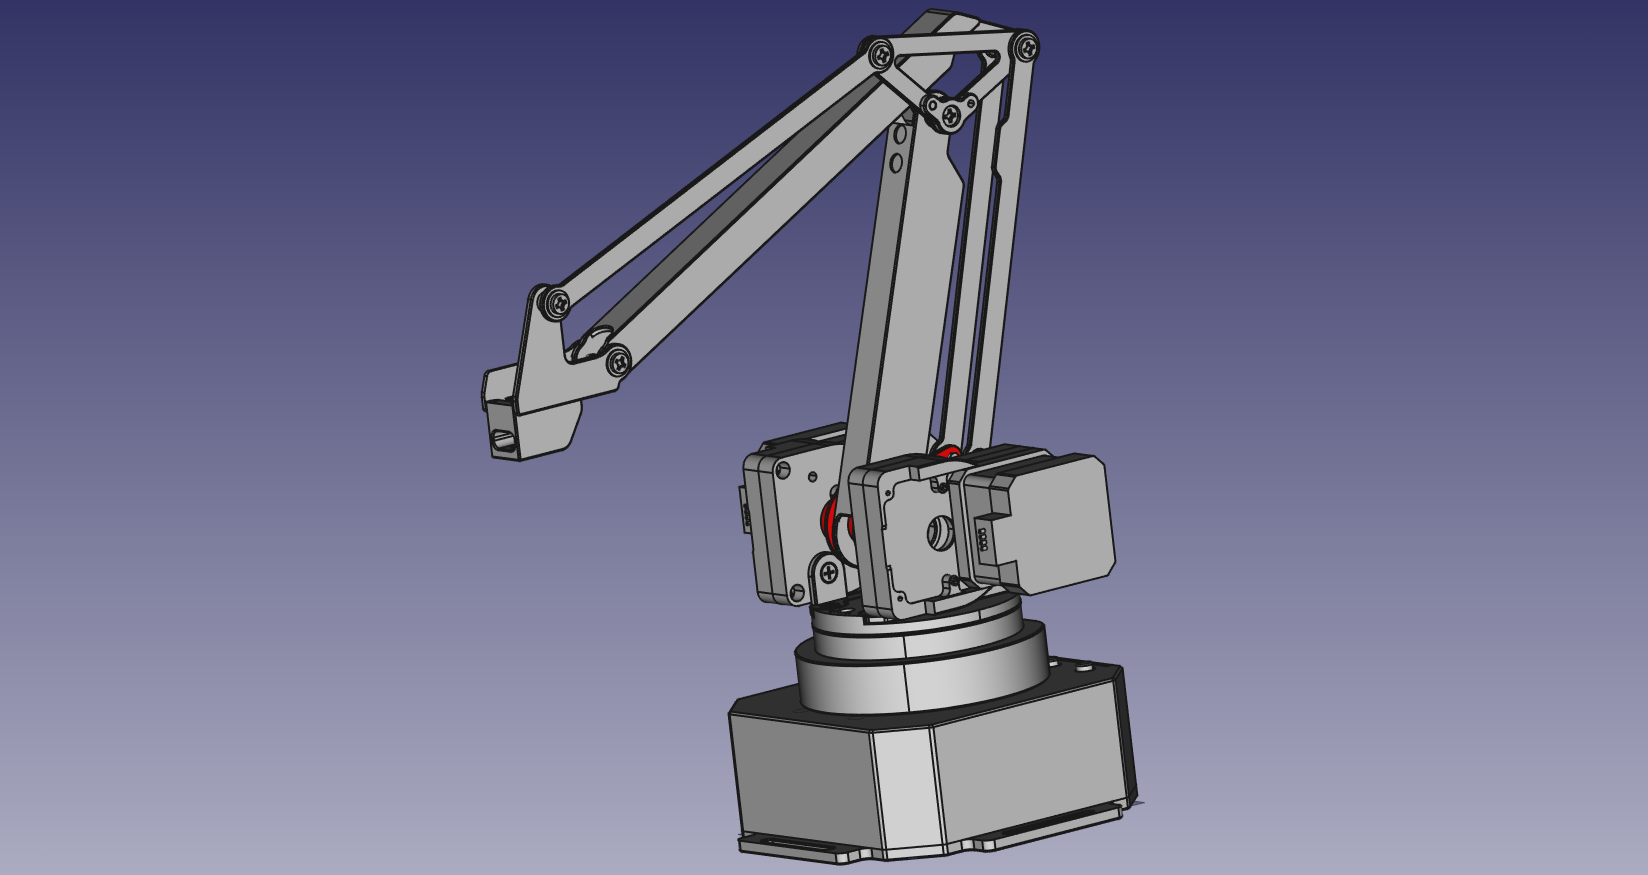
\includegraphics[width=.8\linewidth]{pictures/brazo_vista_3d_inicial.png}
    \caption{Concepto inicial del brazo robótico.}
    \label{fig:manipulador_inicial}
\end{figure}

Las herramientas que han sido empleadas para visualizar y modificar el modelo y posteriormente imprimir las piezas han sido respectivamente FreeCAD y Ultimake Cura.

\begin{figure}[H]
    \centering
    
\includegraphics[width=.45\linewidth]{pictures/freeCAD.jpg}
    \hspace{1cm}
    
\includegraphics[width=.40\linewidth]{pictures/Ultimaker_cura_logo.png}
    \caption{Logotipos de las herramientas utilizadas.}
    \label{fig:herramientas_3d}
\end{figure}

El flujo de trabajo que se ha seguido desde el modelo 3D hasta la impresión de una pieza ha sido el mostrado en la figura \ref{fig:flujo_3d}:

\begin{figure}[H]
    \centering
    \includegraphics[width=.9\linewidth]{pictures/DiagramaImpresión.jpg}
    \caption{Flujo de trabajo del desarrollo y la impresión 3D.}
    \label{fig:flujo_3d}
\end{figure}

Antes de proceder a explicar cada una de las nuevas piezas que se han diseñado, se tomará una de ellas como ejemplo para explicar el proceso de diseño detallado.

Inicialmente se parte de una forma que represente la forma general de la pieza, como un rectángulo o un circulo, para posteriormente añadir detalles. En el caso de la pieza que se usa como ejemplo, tenemos un cuadrado de 120mm de ancho por 120mm de alto y 3 mm de groso.

\begin{figure}[H]
\centering
\subfigure[Plano vacío]{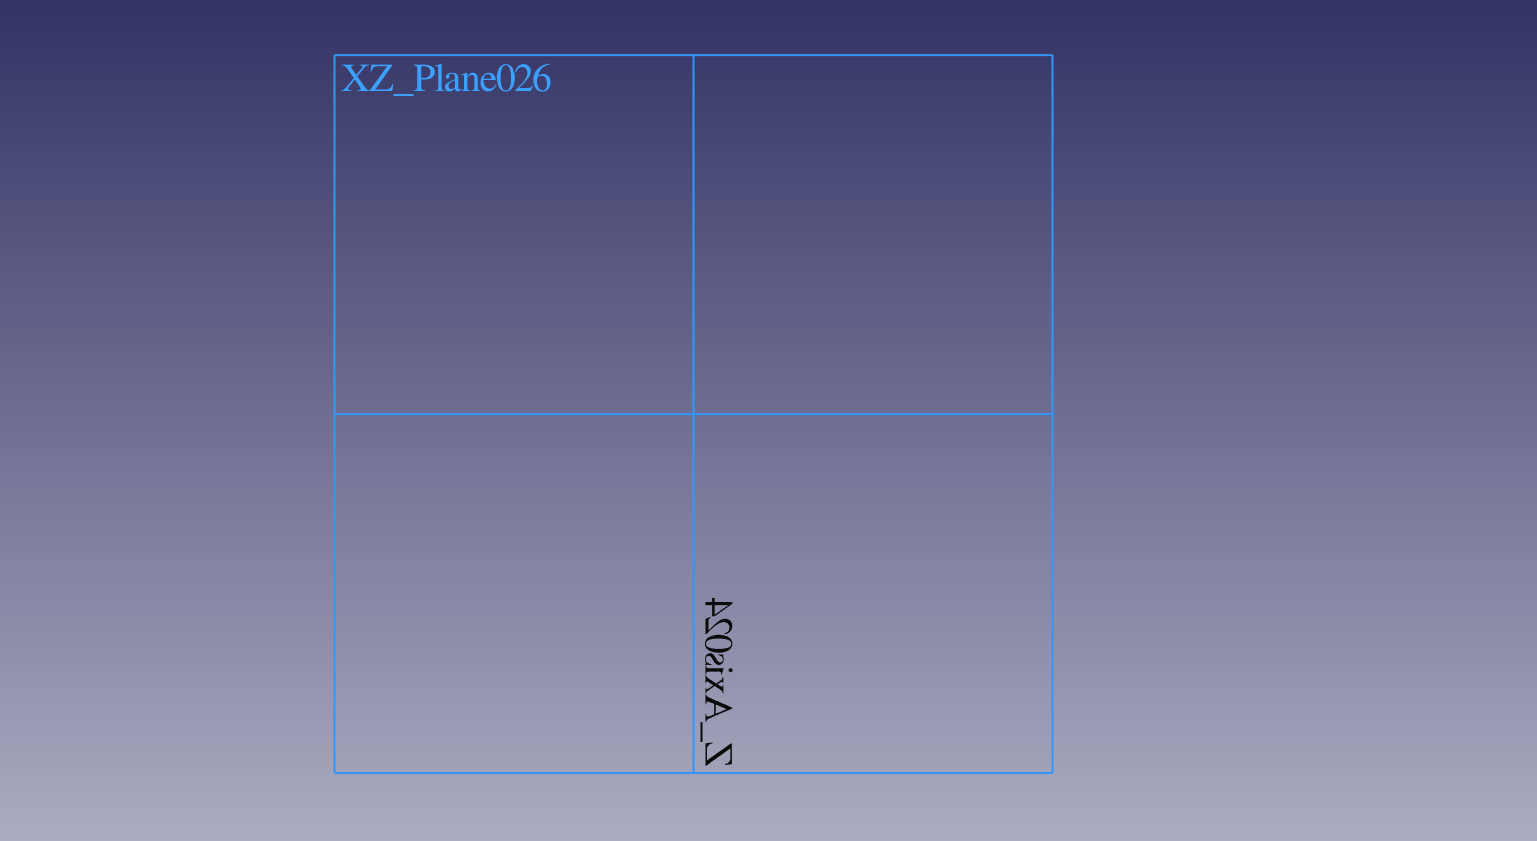
\includegraphics[width=82mm]{pictures/PlanoVacio.png}}
\subfigure[Forma general de la tapa]{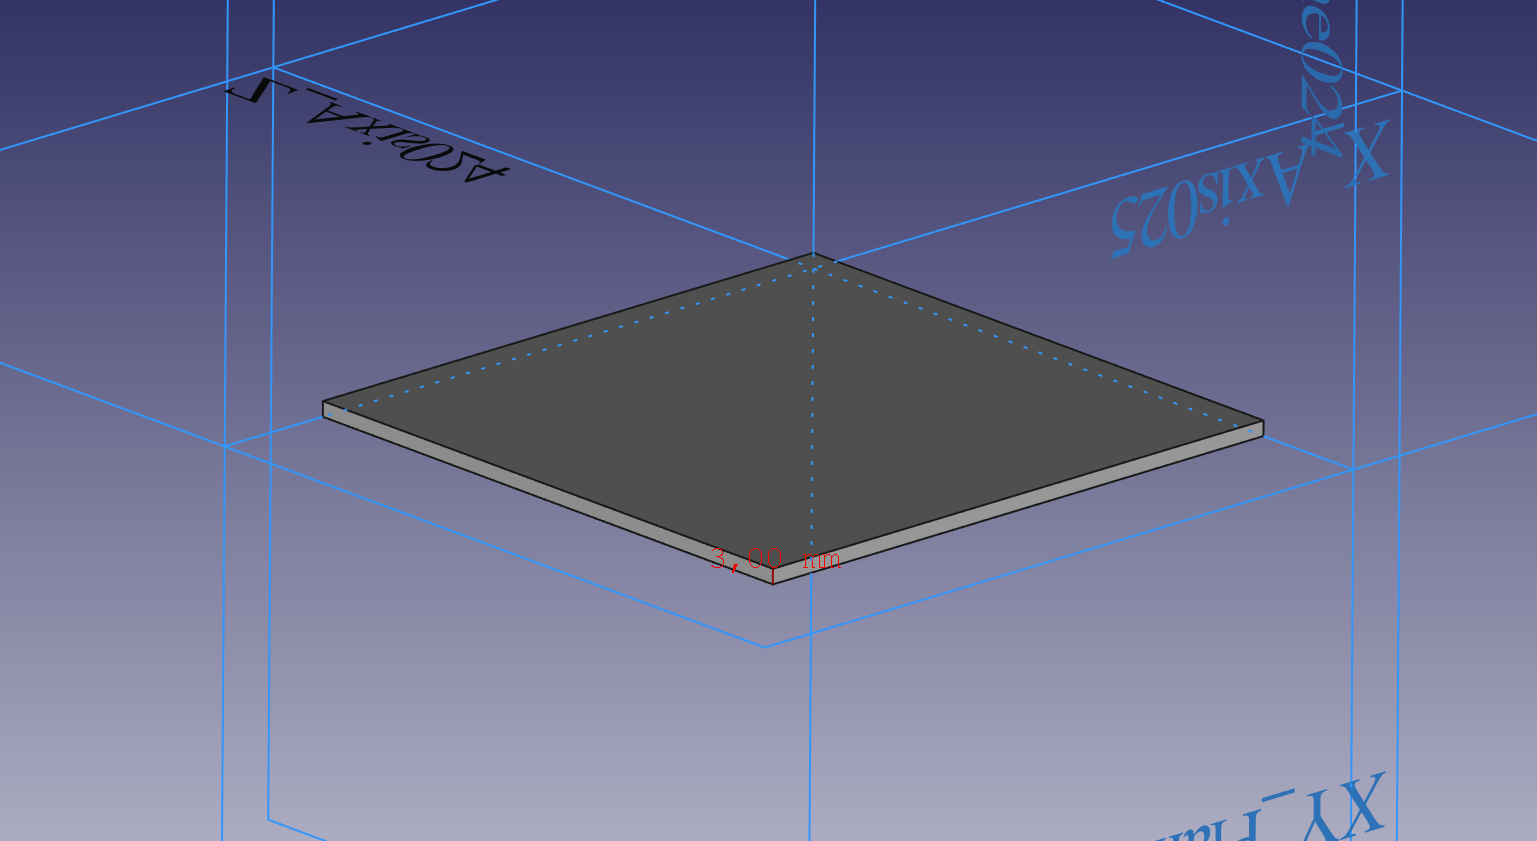
\includegraphics[width=82mm]{pictures/SketchTapaInicial.png}}
\caption{Construcción de la forma general}
\label{fig:forma_general_tapa_superior}
\end{figure}

Tras crear la forma general, añadimos los agujeros en las esquinas para poder atornillar la tapa. Los agujeros tienen un radio de 1,9mm y se distancian de los laterales 3,9mm para hacerlos coincidir con los agujeros de las paredes.

\begin{figure}[H]
\centering
\subfigure[Plano 2D de los agujeros]{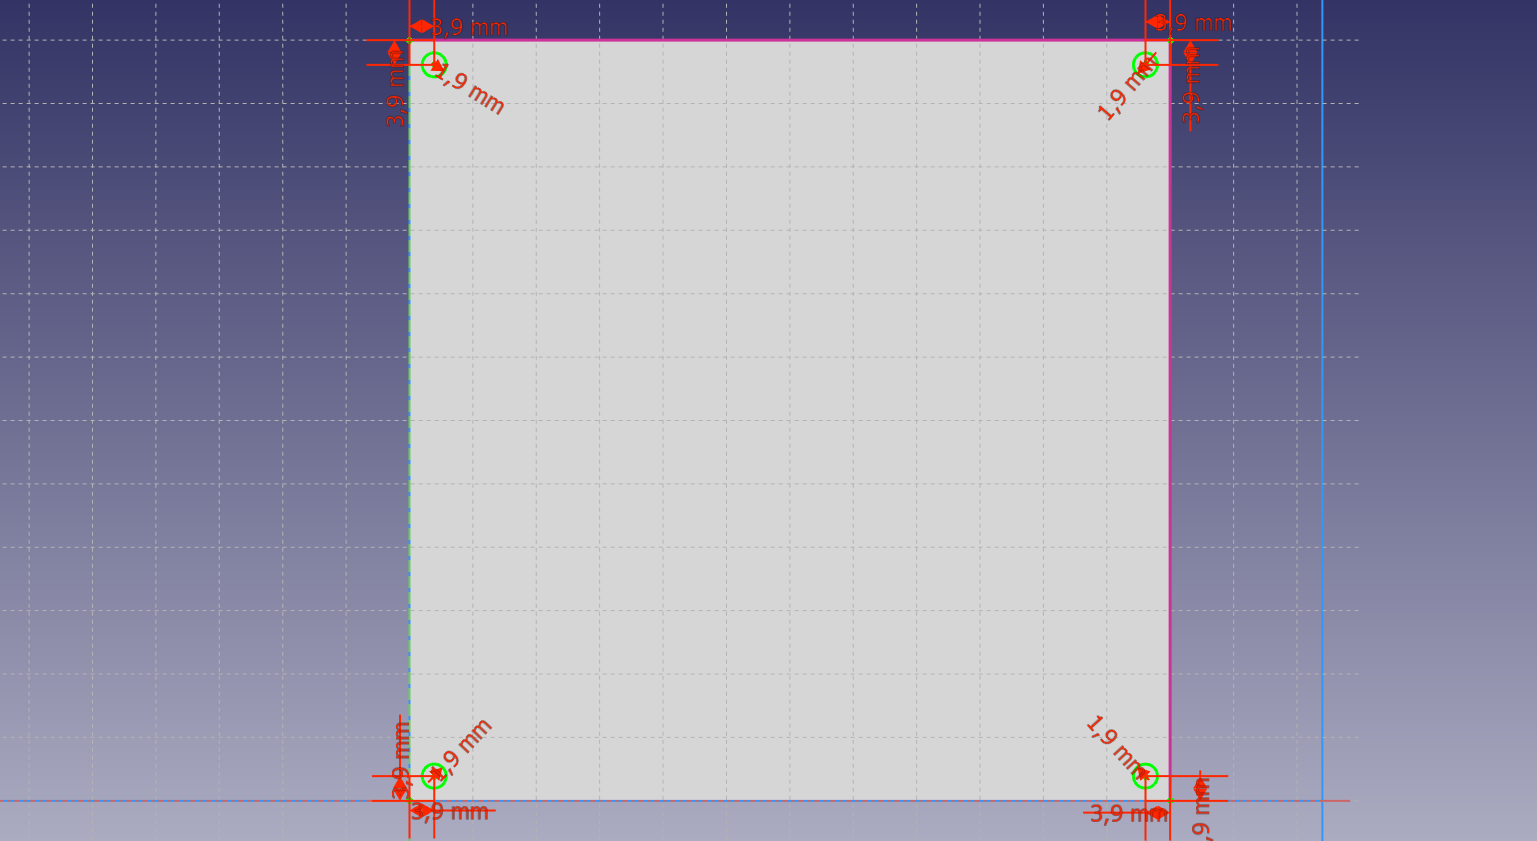
\includegraphics[width=.9\linewidth]{pictures/SketchAgujerosEsquinas.png}}
\subfigure[Detalle de una esquina]{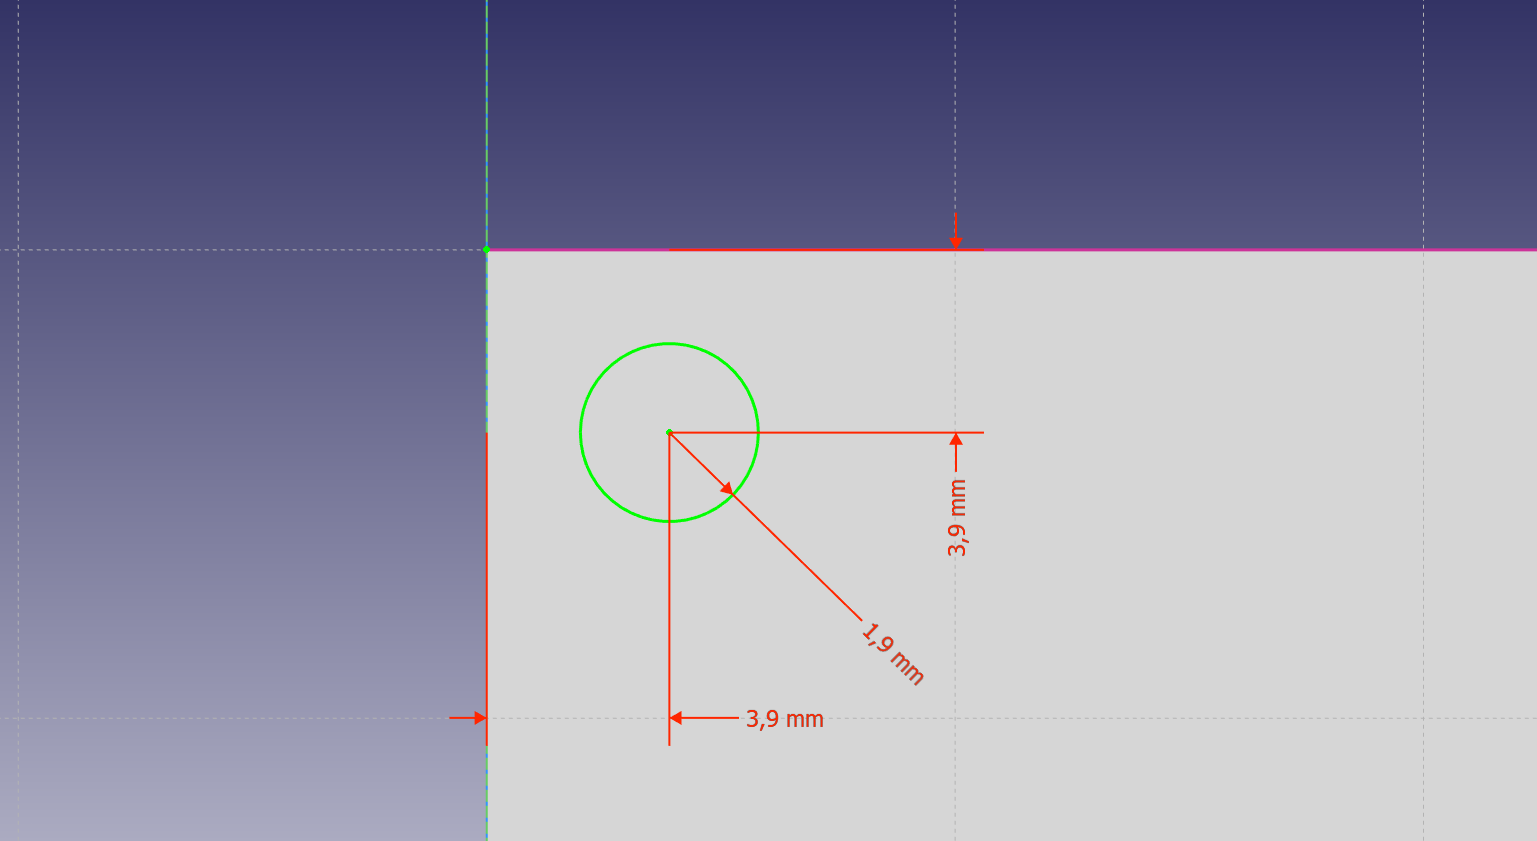
\includegraphics[width=.9\linewidth]{pictures/DetalleAgujerosEsquinas.png}}
\caption{Agujeros para tornillos }
\label{fig:agujeros_tornillos_tapa_superior}
\end{figure}

Tras realizar los agujeros de los exteriores de la pieza, se hace un agujero central y se extruye una torre centrada sobre dicho agujero.

\begin{figure}[H]
\centering
\subfigure[Sketch del agujero central]
{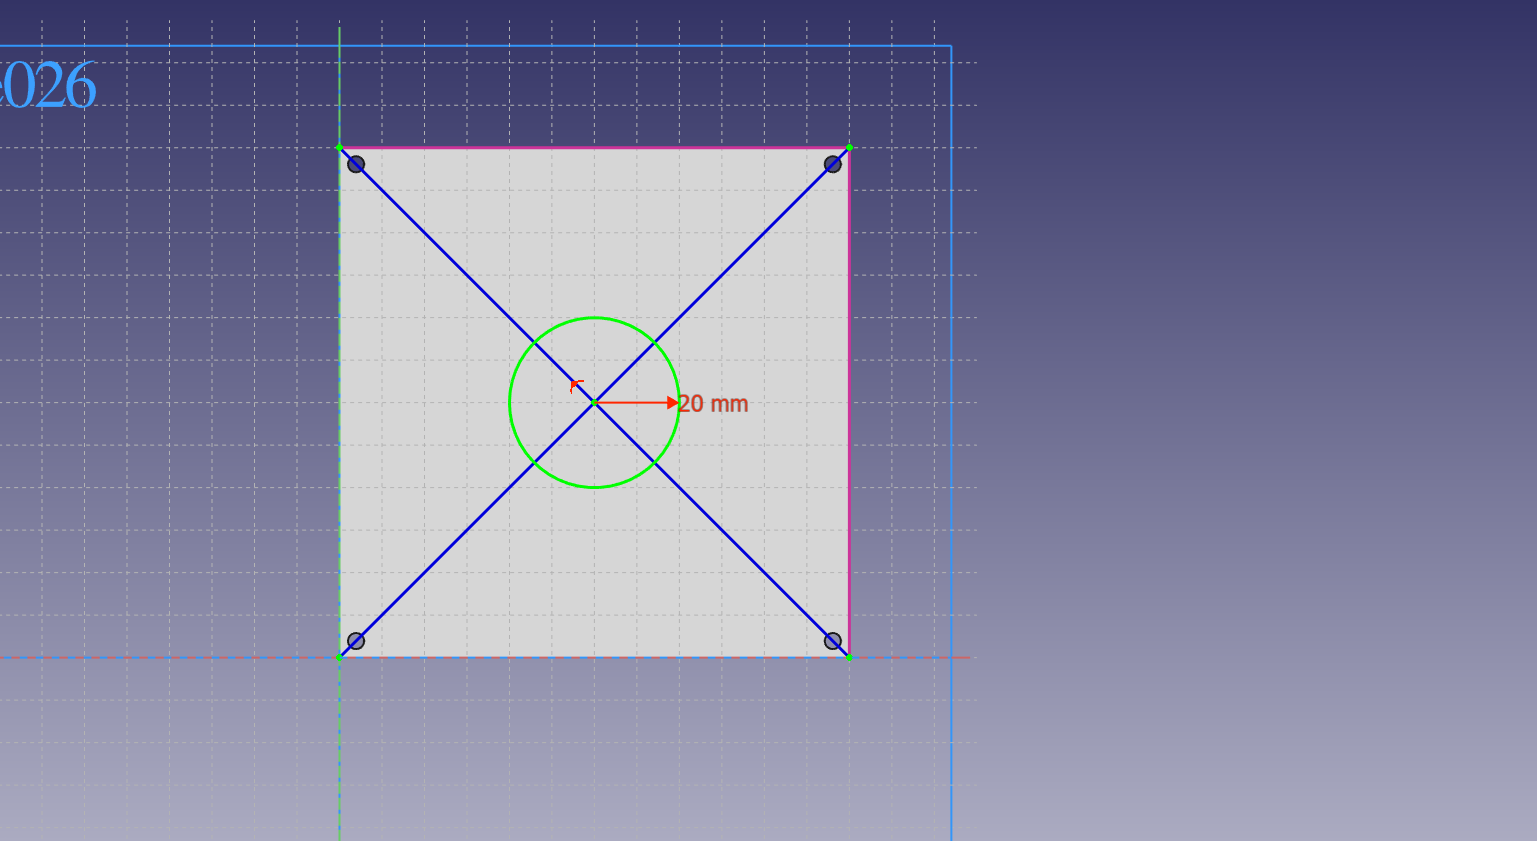
\includegraphics[width=0.9\linewidth]{pictures/SketchAgujeroCentral.png}}
\subfigure[Agujero central sin torre]
{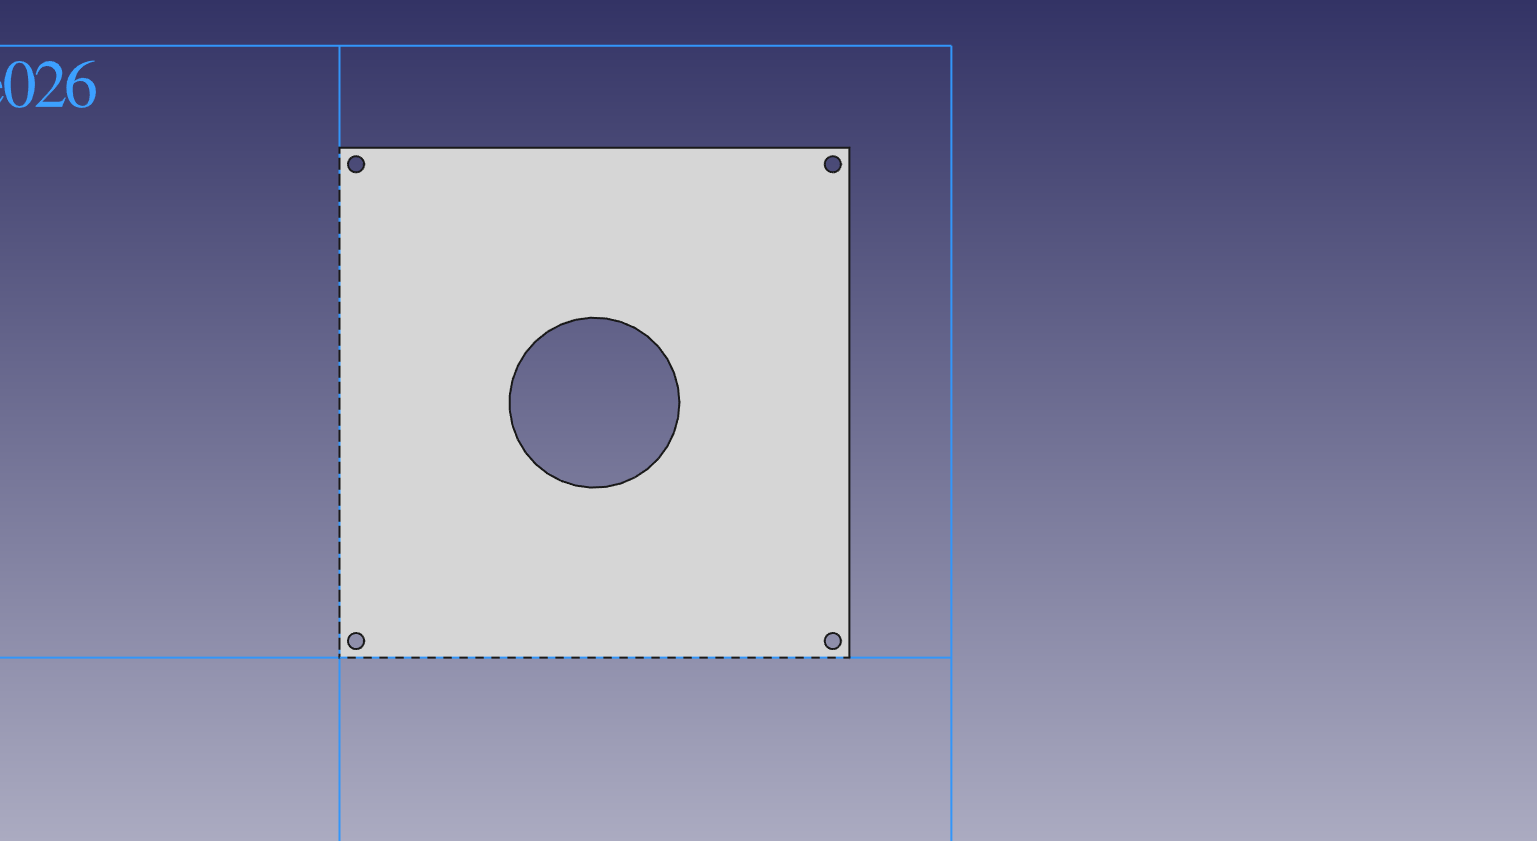
\includegraphics[width=0.9\linewidth]{pictures/AgujeroCentral.png}}
\caption{Agujeros central}
\label{fig:agujeros_central_tapa_superior}
\end{figure}

Tras definir el agujero, se extruye la torre.

\begin{figure}[H]
    \centering
    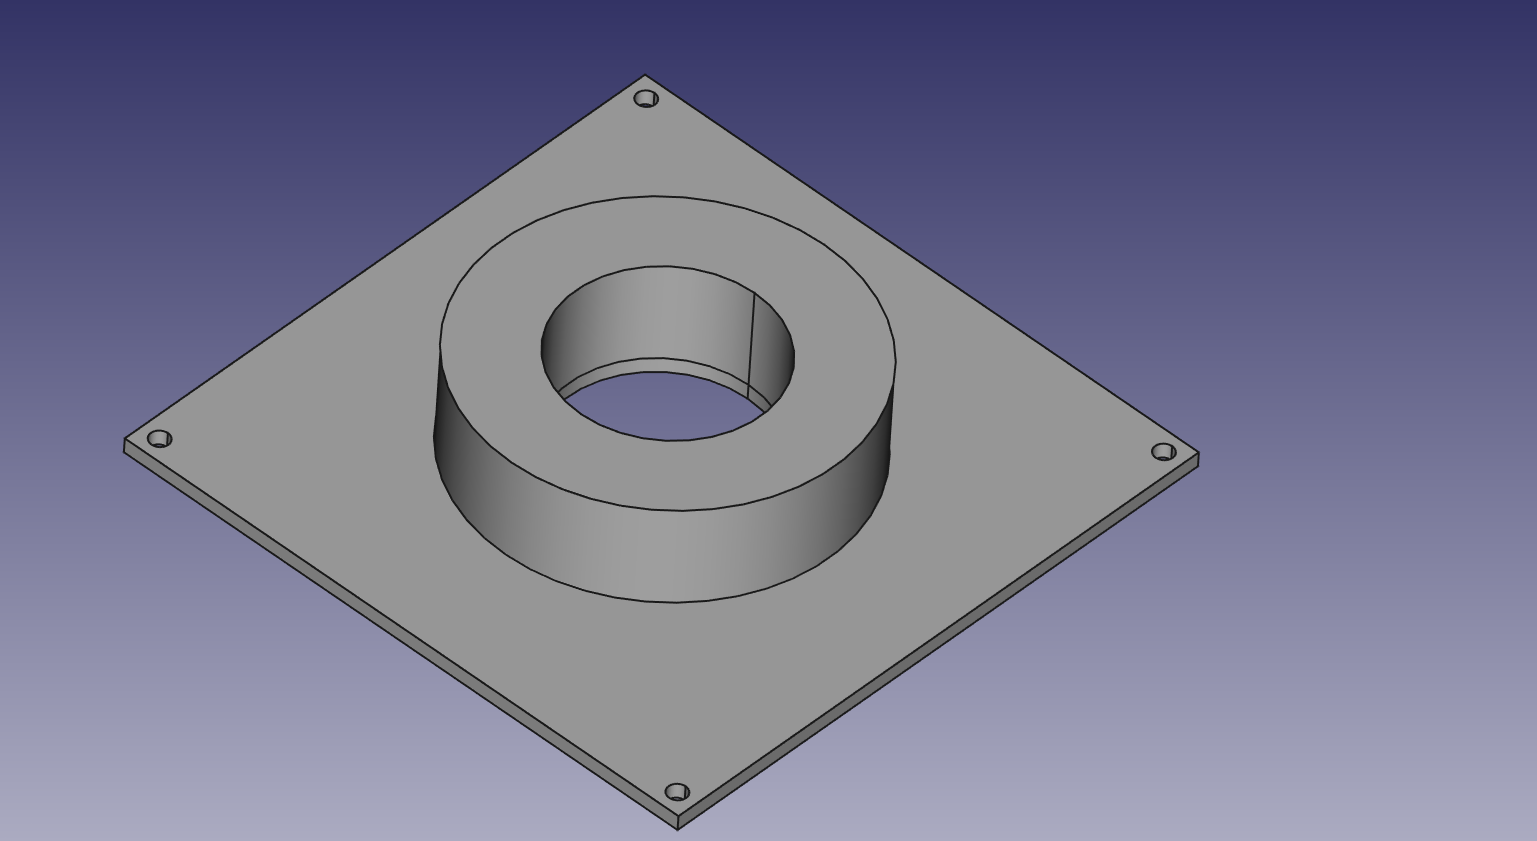
\includegraphics[width=.9\linewidth]{pictures/TorreCentral.png}
    \caption{Tapa con torre central}
    \label{fig:torre_central_tapa_superior}
\end{figure}

A continuación se procede a eliminar material de la torre con
el objetivo de disminuir la superficie de contacto con el disco rotativo y por tanto, eliminar parte del rozamiento.

\begin{figure}[H]
\centering
\subfigure[Sketch del desgaste]
{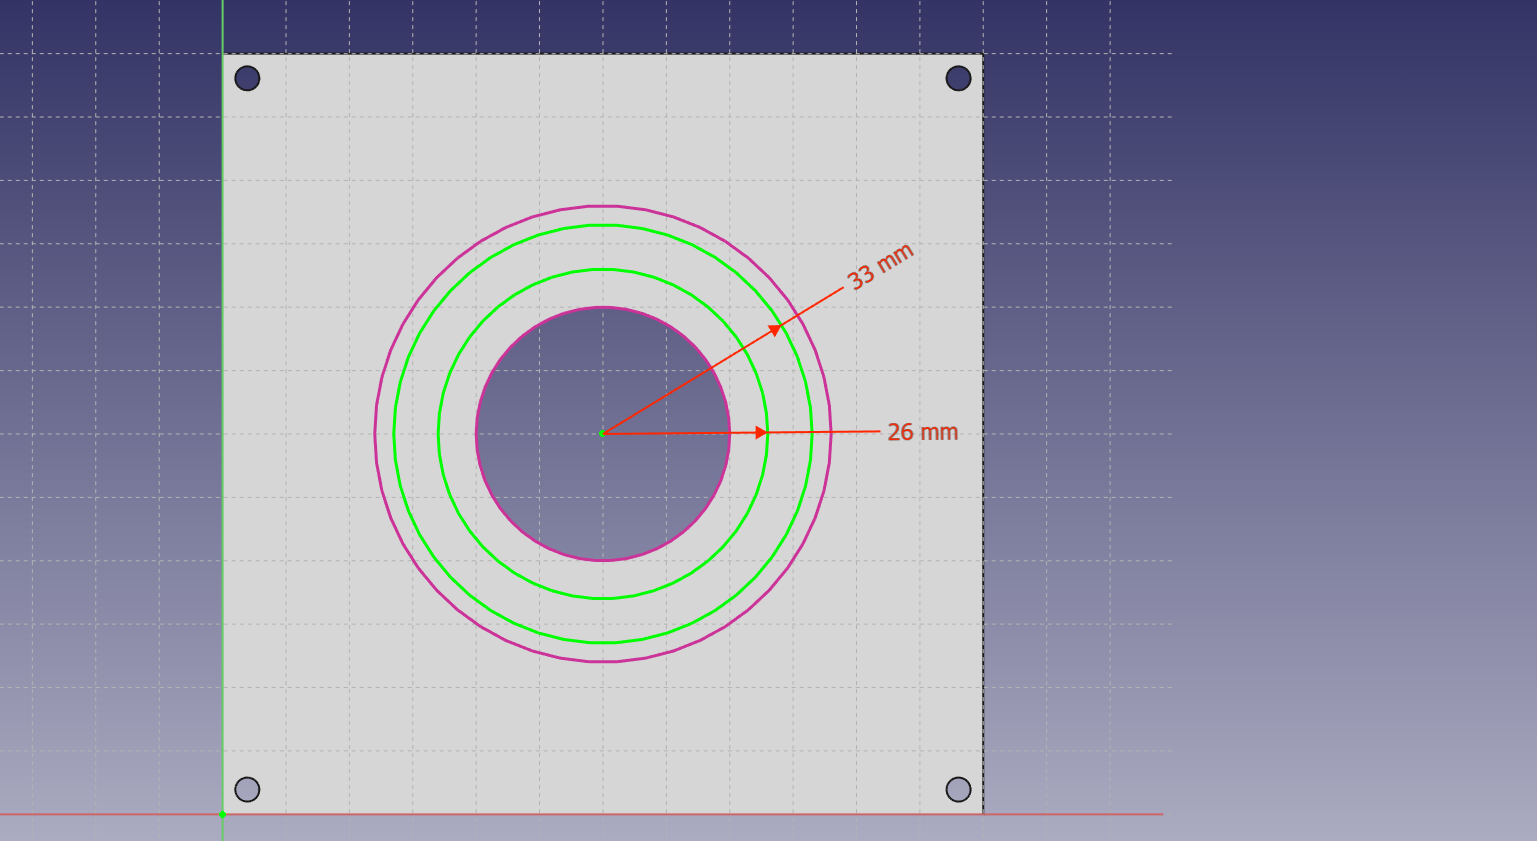
\includegraphics[width=0.9\linewidth]{pictures/SketchAnillo.png}}
\subfigure[Torre central tras el rebaje]
{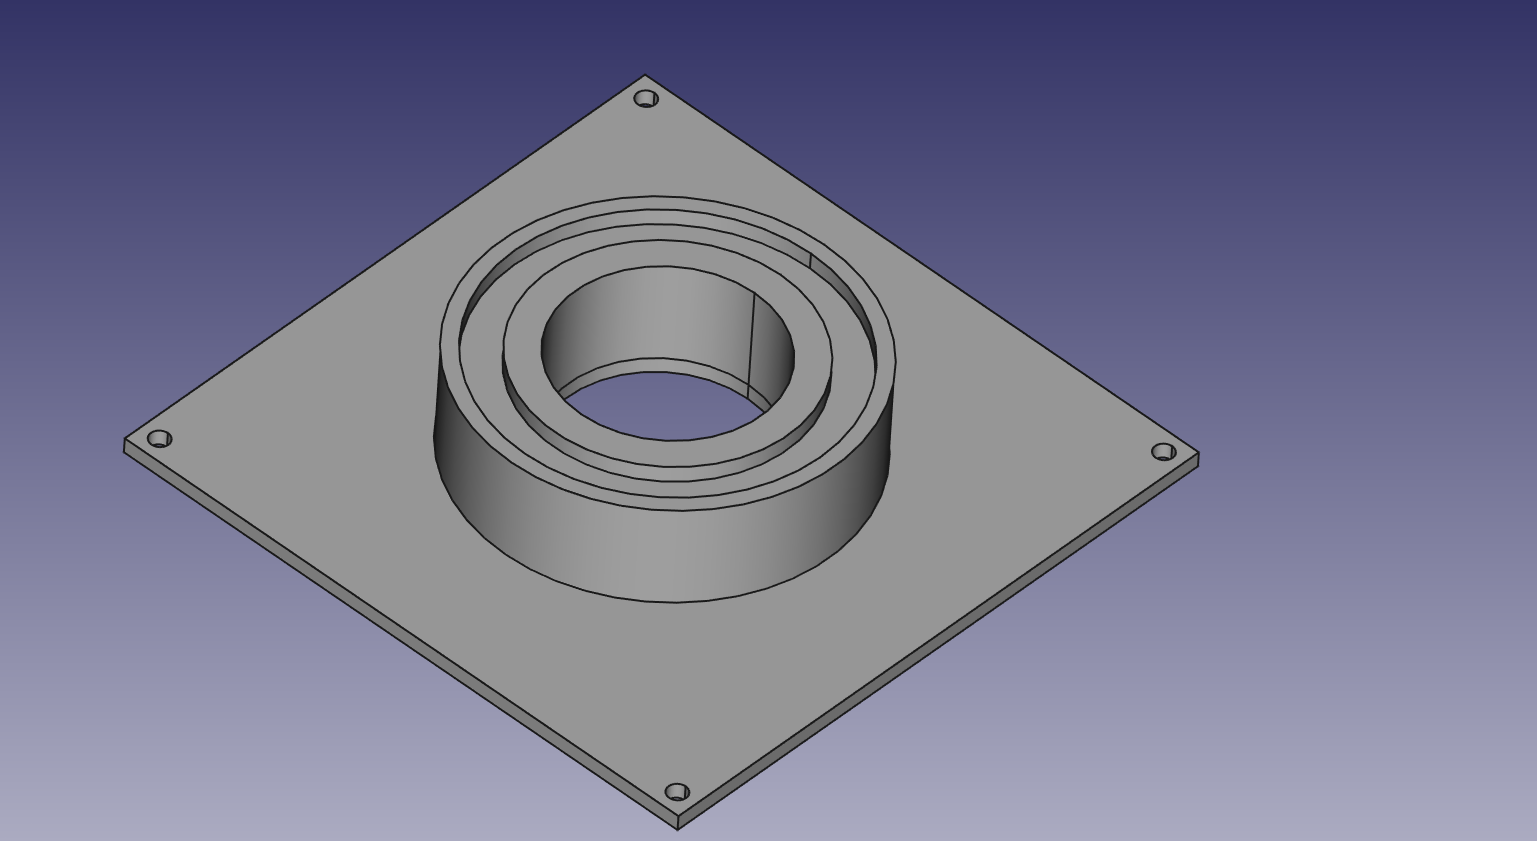
\includegraphics[width=0.9\linewidth]{pictures/Anillo.png}}
\caption{Agujeros central}
\label{fig:anillo_tapa_superior}
\end{figure}

Para disminuir aun mas el rozamiento debido a posibles bordes imperfectos que queden en el disco, se realiza un chaflán en el diámetro interior y exterior.

\begin{figure}[H]
    \centering
    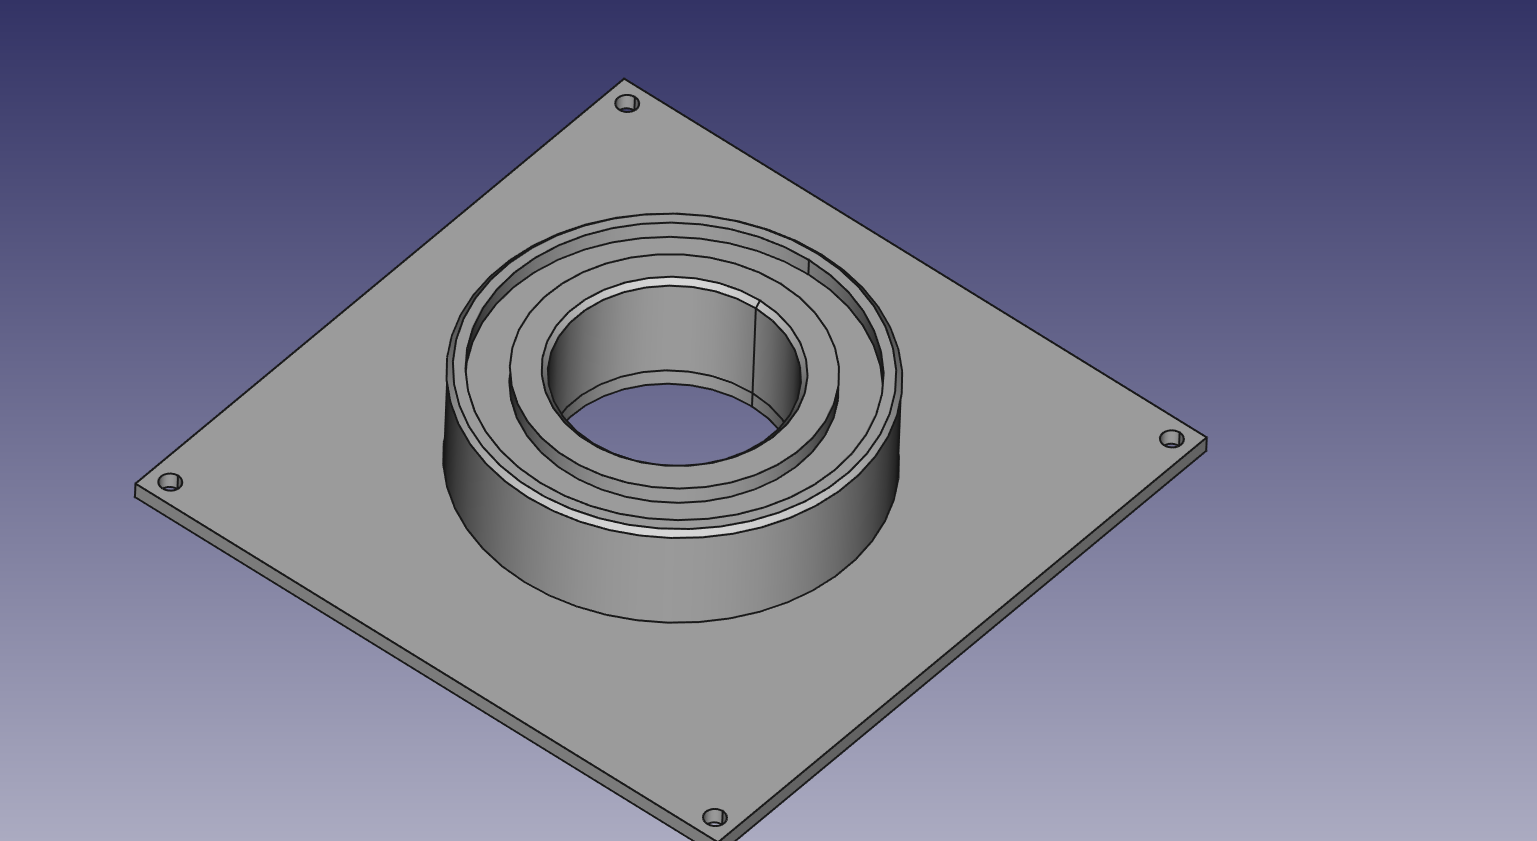
\includegraphics[width=.9\linewidth]{pictures/Chaflanes.png}
    \caption{Torre con chaflanes}
    \label{fig:chaflanes_tapa_superior}
\end{figure}

Finalmente se añade una ranura para que sea posible llevar los cables de los motores exteriores a la placa de control que se haya en la caja.

\begin{figure}[H]
\centering
\subfigure[Sketch de la ranura]
{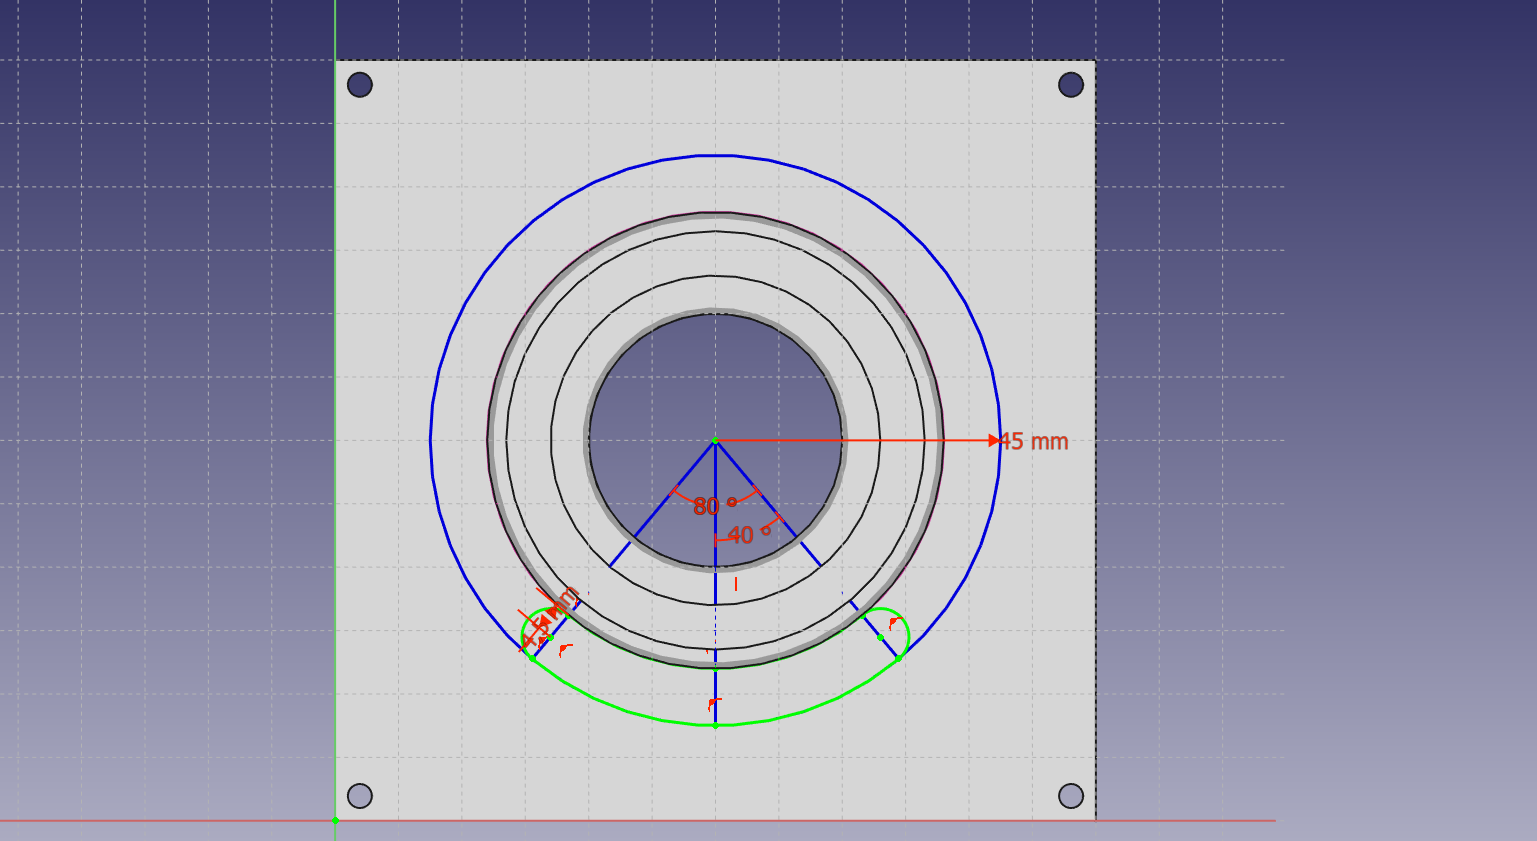
\includegraphics[width=0.9\linewidth]{pictures/SketchAgujeroCables.png}}
\subfigure[Ranura para cables]
{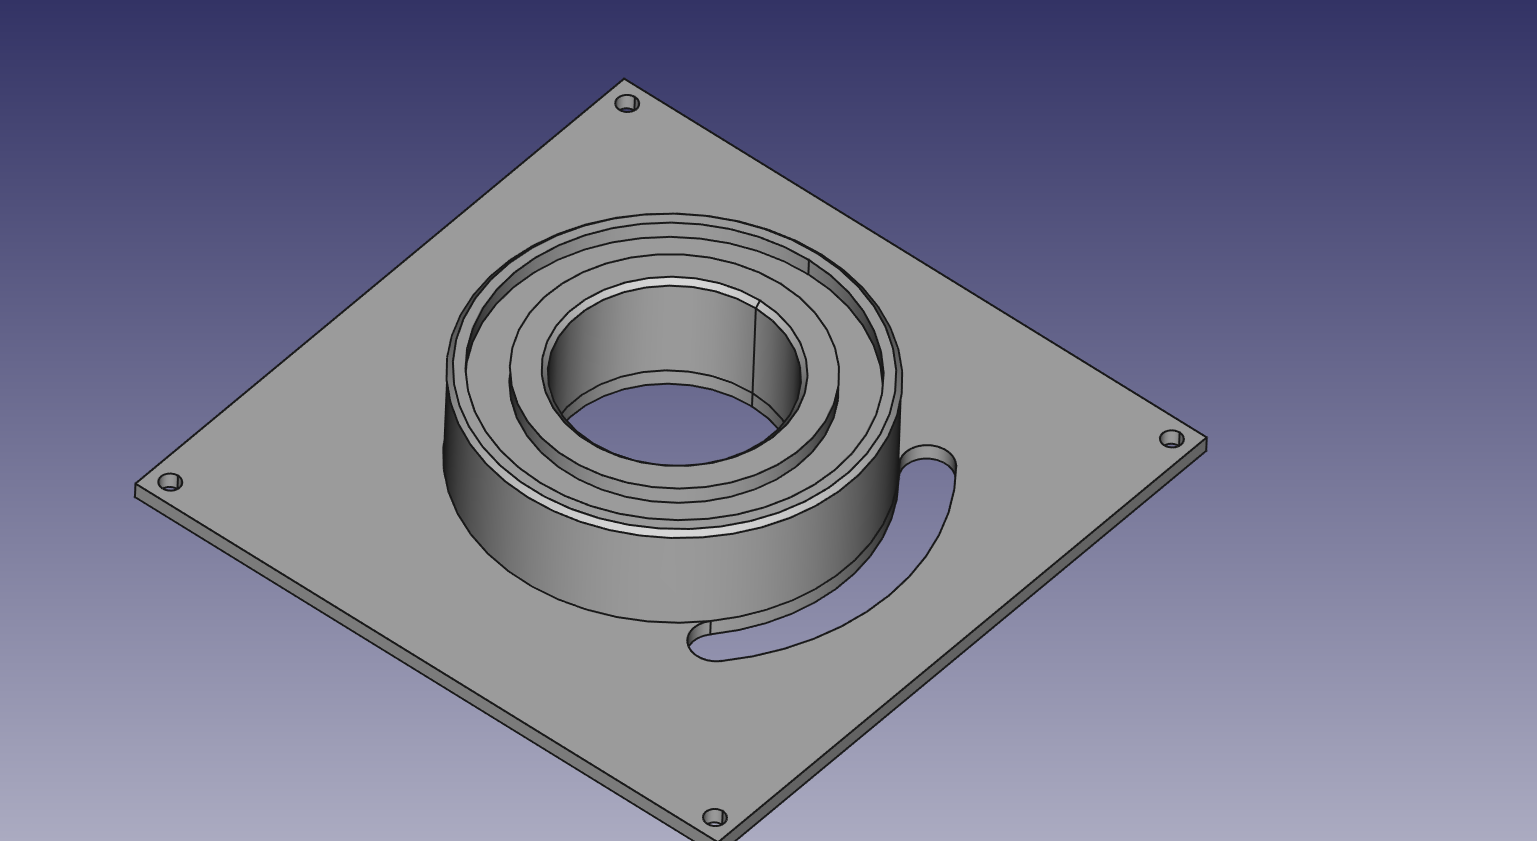
\includegraphics[width=0.9\linewidth]{pictures/AgujeroCables.png}}
\caption{Tapa con ranura para cables}
\label{fig:ranura_cables_tapa_superior}
\end{figure}

Con esto concluimos la explicación del proceso de creación de piezas y pasamos a explicar cada una de las piezas por separado.

A continuación se procederá a explicar la necesidad de remodelar ciertas piezas y los inconvenientes y contratiempos que han surgido durante el modelado y la impresión de estas.

En primer lugar se explicará la caja que alberga la placa de control y uno de los motores.

La placa de control del brazo robótico no es la misma que en el caso del $\mu$Arm de UFACTORY. Además, los motores que se han empleado en este proyecto son servomotores con carcasa y sistema de sujeción distintos a los motores paso a paso del $\mu$Arm. Debido a estos dos factores se ha tenido que diseñar nuevas partes para la base del brazo robótico.

 Mas concretamente, la necesidad de rediseñar esta parte es debida a que la base original era demasiado pequeña en superficie para permitir introducir la placa de control. Además, el servomotor no podría haber cabido junto con la placa ya que la altura era insuficiente. Por otro lado los sistemas de sujeción presentes en la caja existente no podían ser empleados para la placa de control desarrollada en este proyecto.
 
 \begin{figure}[H]
    \centering
    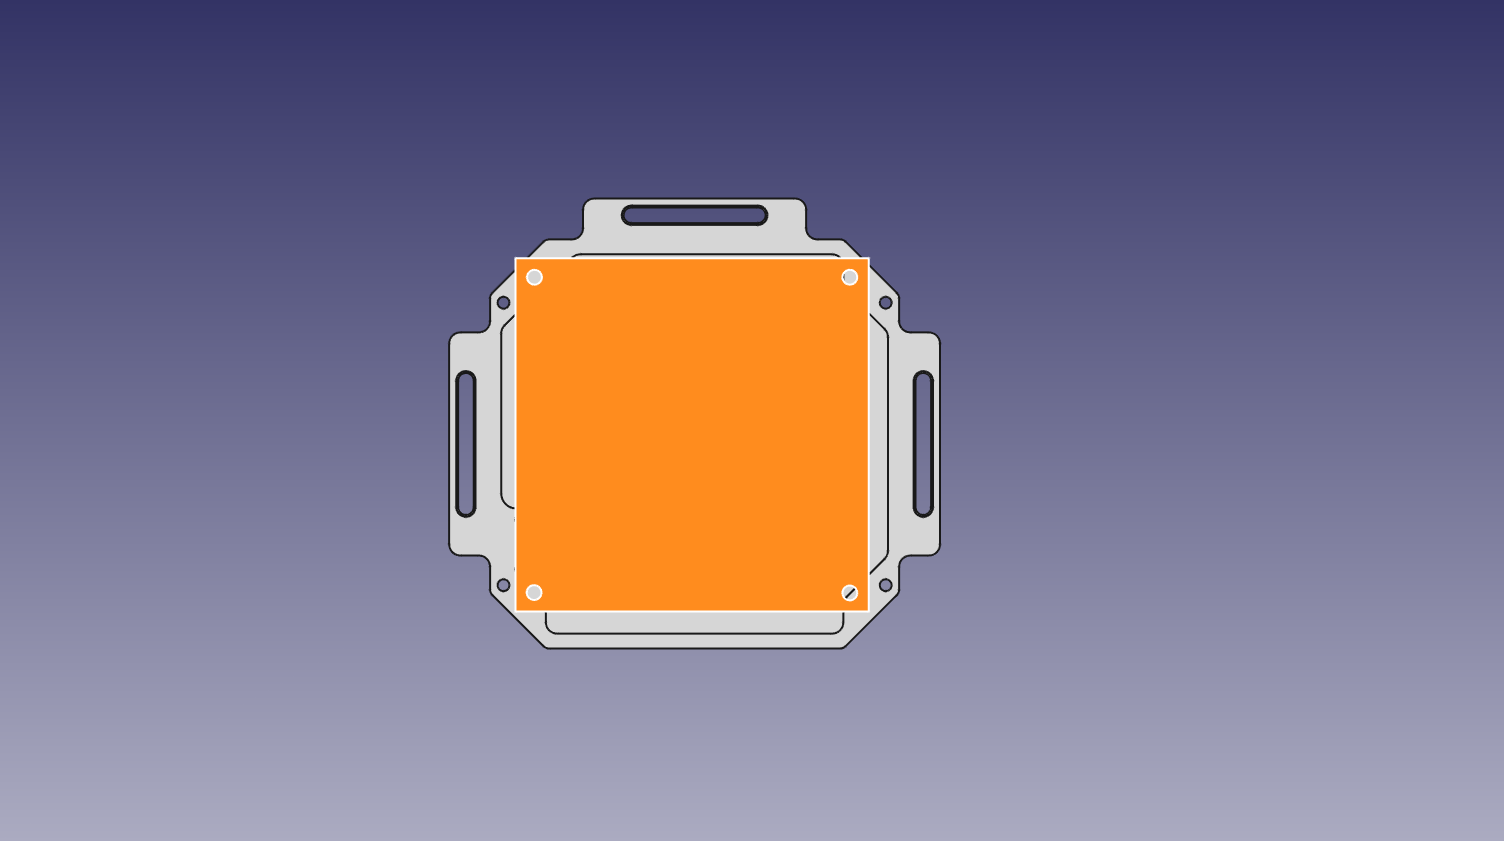
\includegraphics[width=.9\linewidth]{pictures/PlacaYBase.png}
    \caption{Proyección de la placa de control (naranja) sobre la base original del $\mu$Arm (gris)}
    \label{fig:placa_y_base_antiguas}
\end{figure}


 \begin{figure}[H]
    \centering
    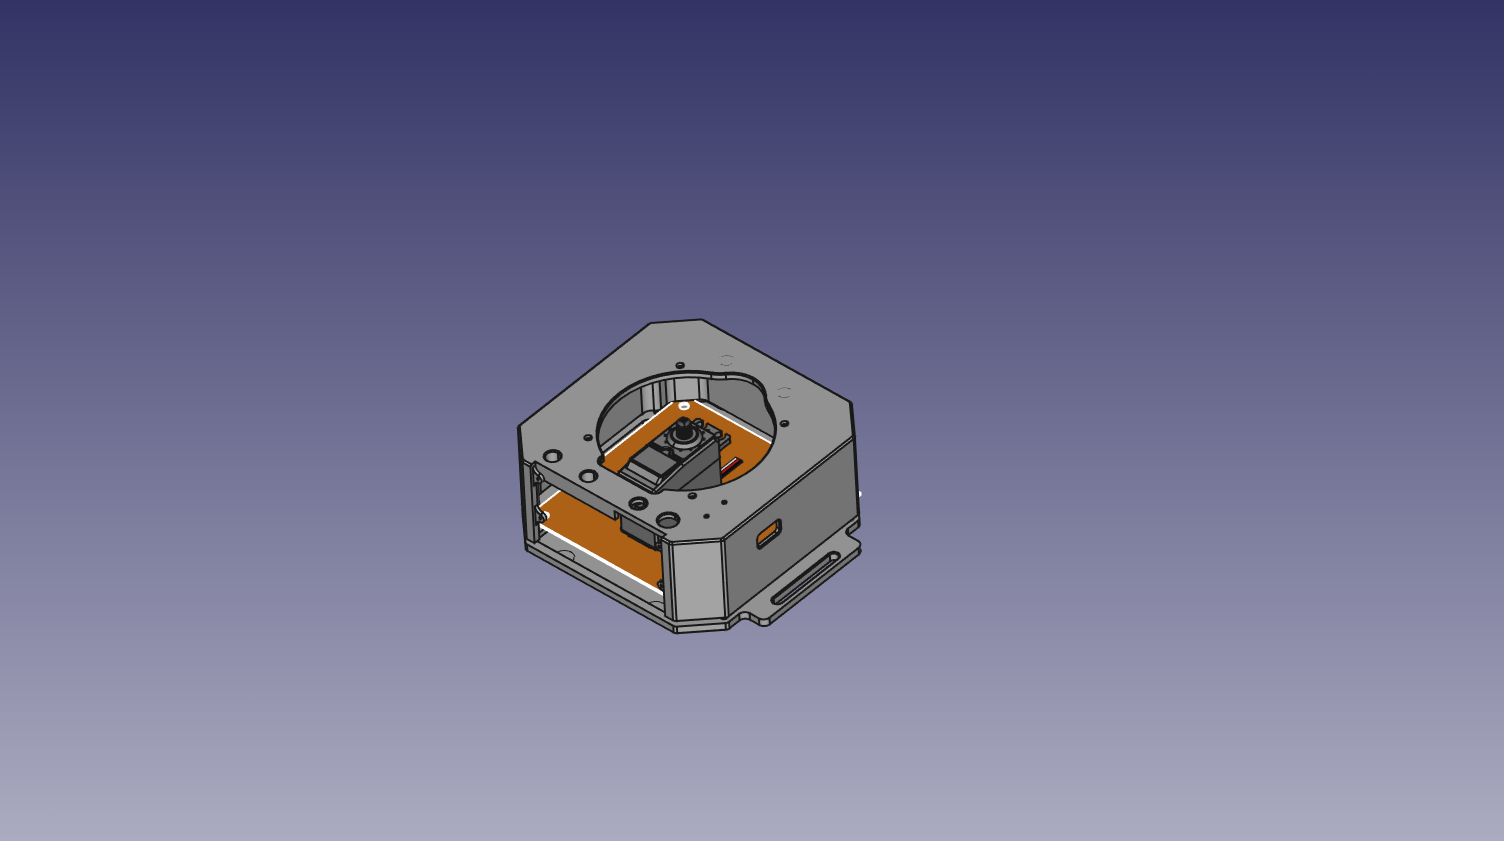
\includegraphics[width=.9\linewidth]{pictures/PlacaMotorYParedes1.png}
    \caption{Placa y motor dentro de la caja original del $\mu$Arm}
    \label{fig:placa_motor_y_paredes1}
\end{figure}

Como se observa en la figura \ref{fig:placa_motor_y_paredes1} el motor sobresale por encima de las paredes y no hay ninguna manera de sujetarlo a estas o a la base.

Para solucionar los anteriores problemas se diseña una nueva base en la que se pueda encajar la placa, además de unas paredes lo suficientemente altas para poder introducir el motor junto con la placa.

 \begin{figure}[H]
    \centering
    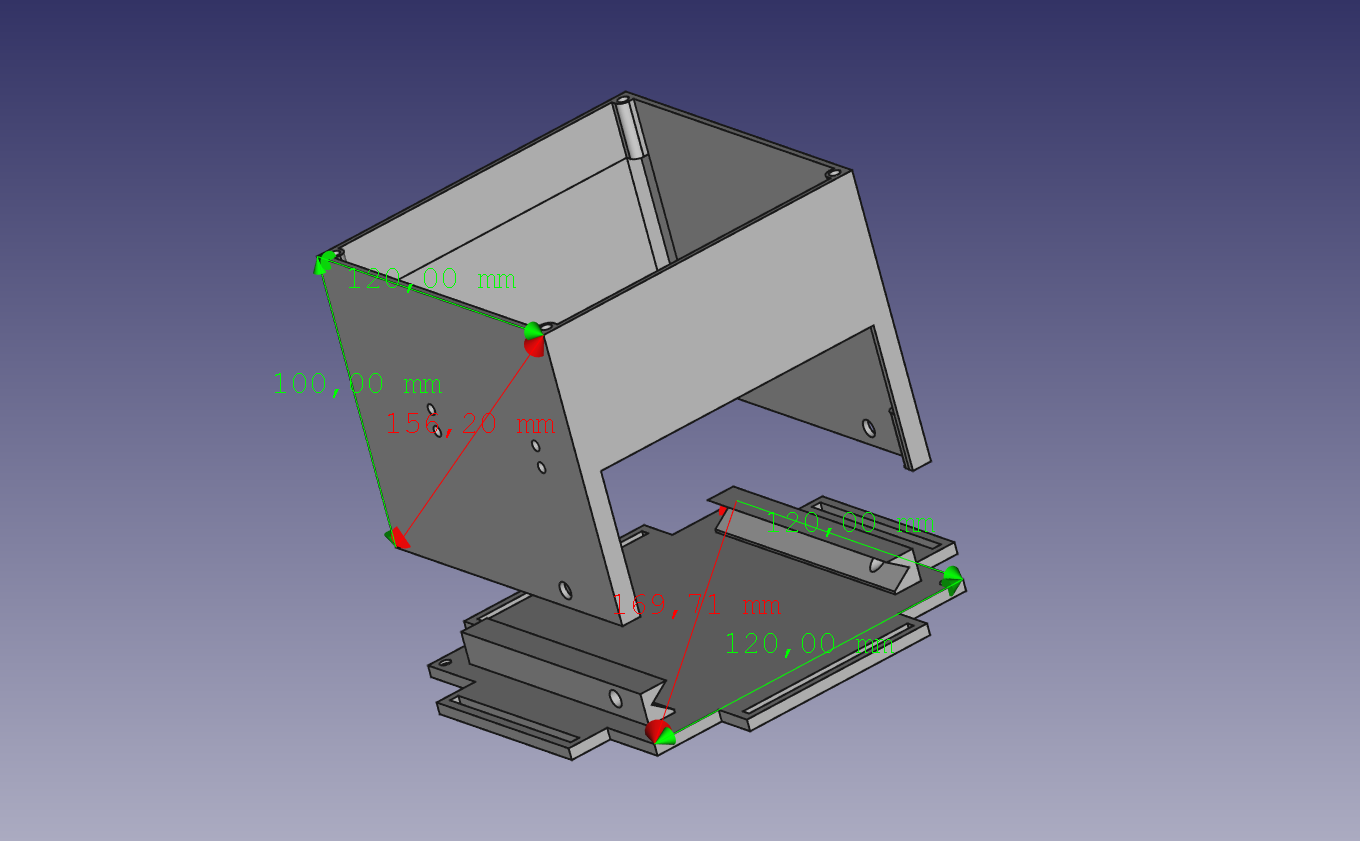
\includegraphics[width=.9\linewidth]{pictures/paredesybasenuevas.png}
    \caption{Base y paredes tras realizar las modificaciones necesarias}
    \label{fig:placa_y_paredes_nuevas}
\end{figure}

Inicialmente las paredes de la caja se habían diseñado con un grosor de 2mm. Tras una serie de pruebas se concluyo que dicho grosor no era suficiente para proporcionar resistencia y estabilidad suficiente, por tanto, se opto por un grosor de 3mm en la versión final.

En la base se observan los raíles que servirán para introducir y retirar la placa de la estructura. 

Se ha optado por un sistema de raíles en vez de una sujeción convencional ya que de esta manera se consigue una mayor versatilidad a la hora de extraer e introducir la placa en labores de depuración y construcción. 

Además, debido al escaso espacio dentro de la caja, se hace prácticamente imposible la introducción de las herramientas necesarias para atornillar la placa a la estructura. Gracias al sistema de raíles se evita desmontar ciertas piezas al intentar introducir o extraer la placa.

Después de que la placa sea insertada en estos carriles, se asegura su posición mediante los agujeros laterales que pueden observarse en la figura \ref{fig:placa_y_paredes_nuevas}.

 \begin{figure}[H]
    \centering
    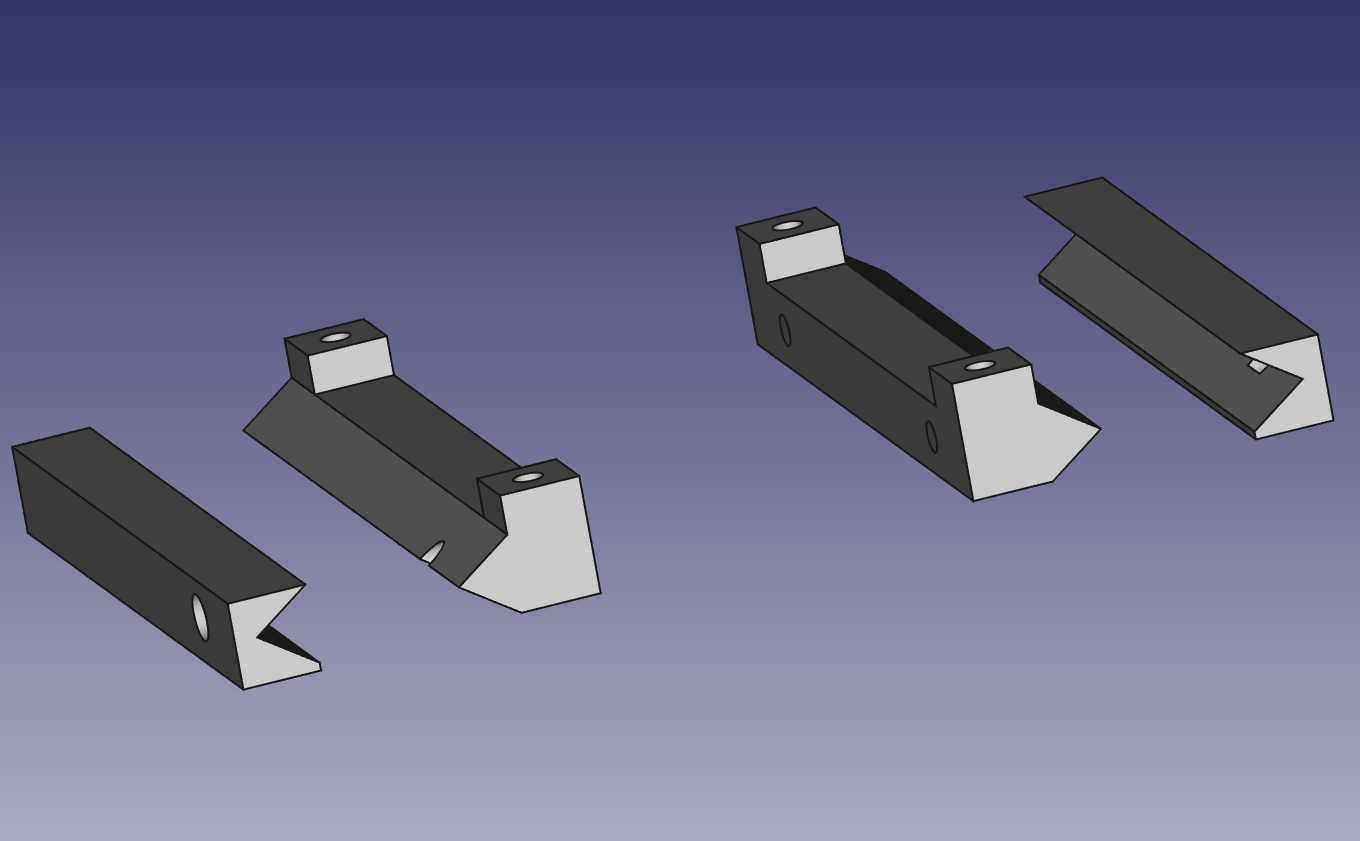
\includegraphics[width=.9\linewidth]{pictures/railes.png}
    \caption{Sistema de raíles de la placa}
    \label{fig:railes_placa}
\end{figure}

En la figura \ref{fig:railes_placa} se observan las piezas que se añadirán a la placa de control para poder deslizar esta sobre los carriles. En el exterior de la imagen aparecen los carriles presentes en la base de la caja, donde se puede ver que, al estar la placa completamente introducida en los carriles, los agujeros del carril y del raíl se posición de tal manera que se permite introducir un pasador que asegura la posición de la placa.

Debido a que tanto los raíles como los carriles se fabricaron con unas medidas teóricas, extraídas del diseño físico inicial de la placa, resulto que el ensamblaje físico no era posible.

Para solucionar este problemas se desplazaron los agujeros por los que se unía el raíl a la placa. Esto se observa en la figura \ref{fig:railes_placa_final}

 \begin{figure}[H]
    \centering
    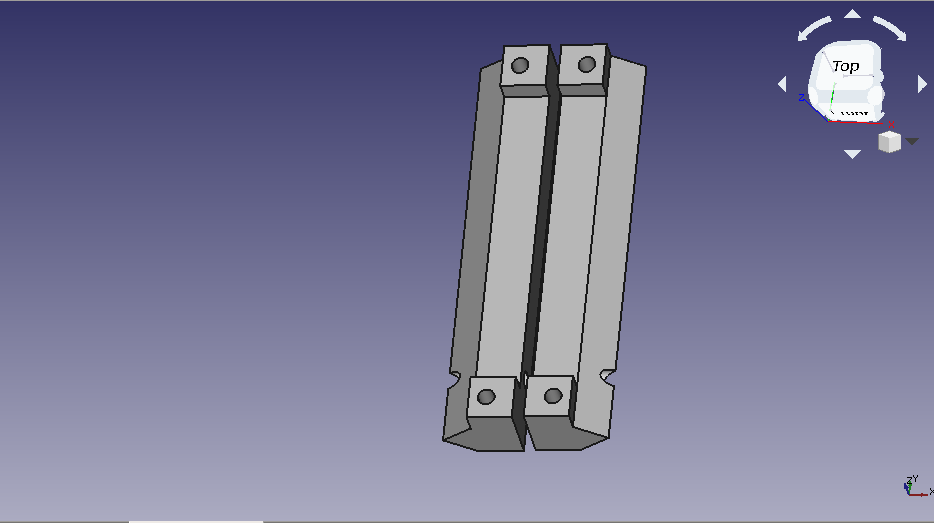
\includegraphics[width=.9\linewidth]{pictures/RailesBien.png}
    \caption{Versión final de los carriles}
    \label{fig:railes_placa_final}
\end{figure}

Por otro lado, para poder sujetar el motor que moverá el brazo alrededor del eje vertical se ha tenido que diseñar la siguiente pieza.

 \begin{figure}[H]
    \centering
    \includegraphics[width=.9\linewidth]{pictures/sujecciónMotor.png}
    \caption{Pieza de sujeción del motor}
    \label{fig:sujecion_motor}
\end{figure}

Esta pieza se atornilla a las paredes de la caja y empleando las solapas del motor, este se atornilla en el centro de la pieza como se puede ver en la figura \ref{fig:pieza_sujecio_en_caja}.

 \begin{figure}[H]
    \centering
    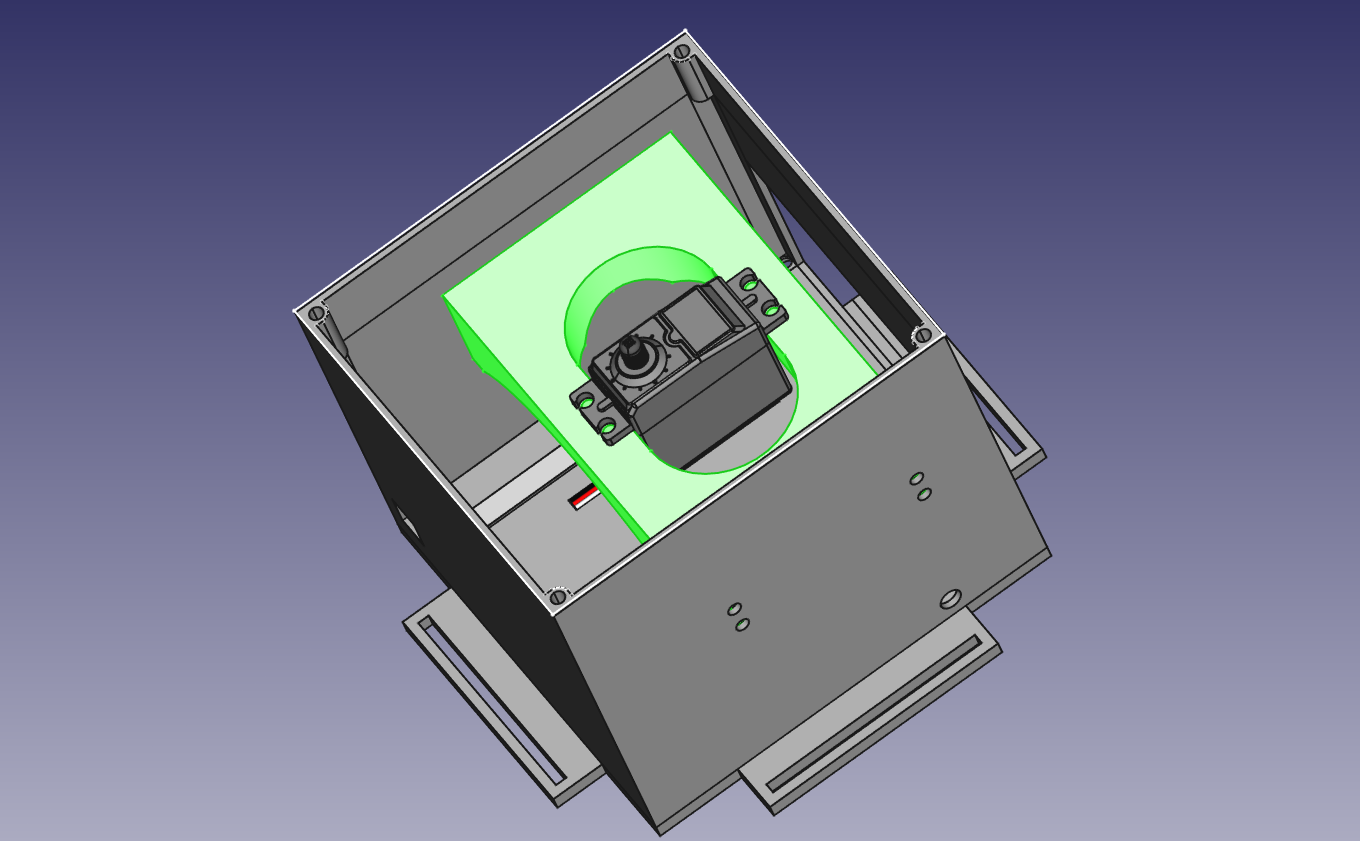
\includegraphics[width=.9\linewidth]{pictures/cajaConMotor.png}
    \caption{Pieza de sujeción del motor (verde) dentro de la caja}
    \label{fig:pieza_sujecio_en_caja_resaltada}
\end{figure}

La pieza que sujeta el motor se diseño con un grosor de las paredes de 2mm. Como se ha descrito anteriormente este grosor 

Dado que el tamaño de la base y de las paredes ha cambiado, la tapa superior debe también ser modificada para adaptar su tamaño y su sistema de sujeción a los nuevos diseños

 \begin{figure}[H]
    \centering
    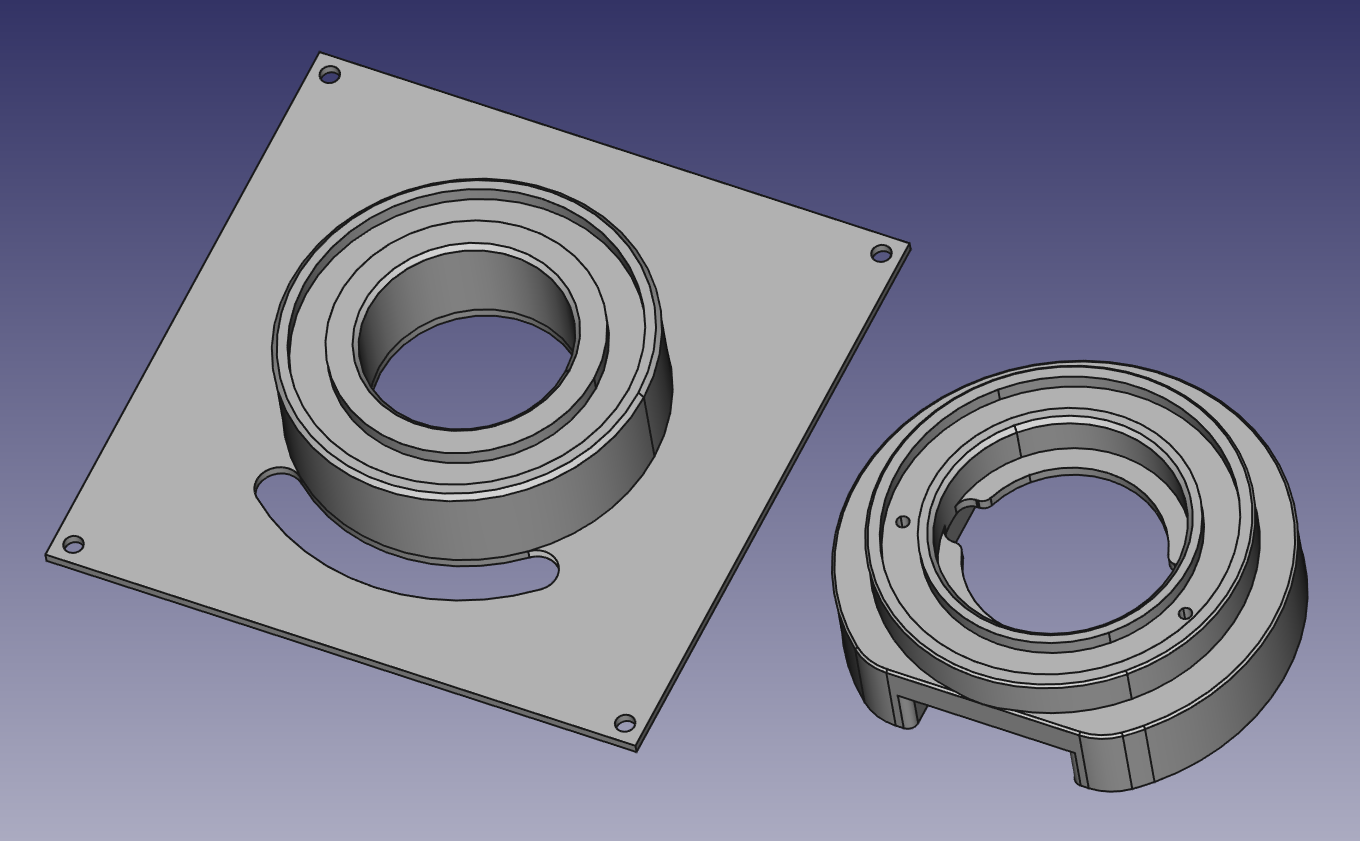
\includegraphics[width=.9\linewidth]{pictures/DosTapas.png}
    \caption{Tapa original (derecha) junto a la tapa modificada (izquierda)}
    \label{fig:tapas_caja}
\end{figure}

En la figura \ref{fig:tapas_caja} se observa que en la parte superior las diferencias entre ambas piezas son mínimas respetándose los diámetros del disco exterior e interior sobre los que descansará la base giratoria.

En la figura \ref{fig:tapas_caja_con_disco} podemos observar como la base giratoria descansa sobre los anillos superiores y se inserta dentro de la tapa.

 \begin{figure}[H]
    \centering
    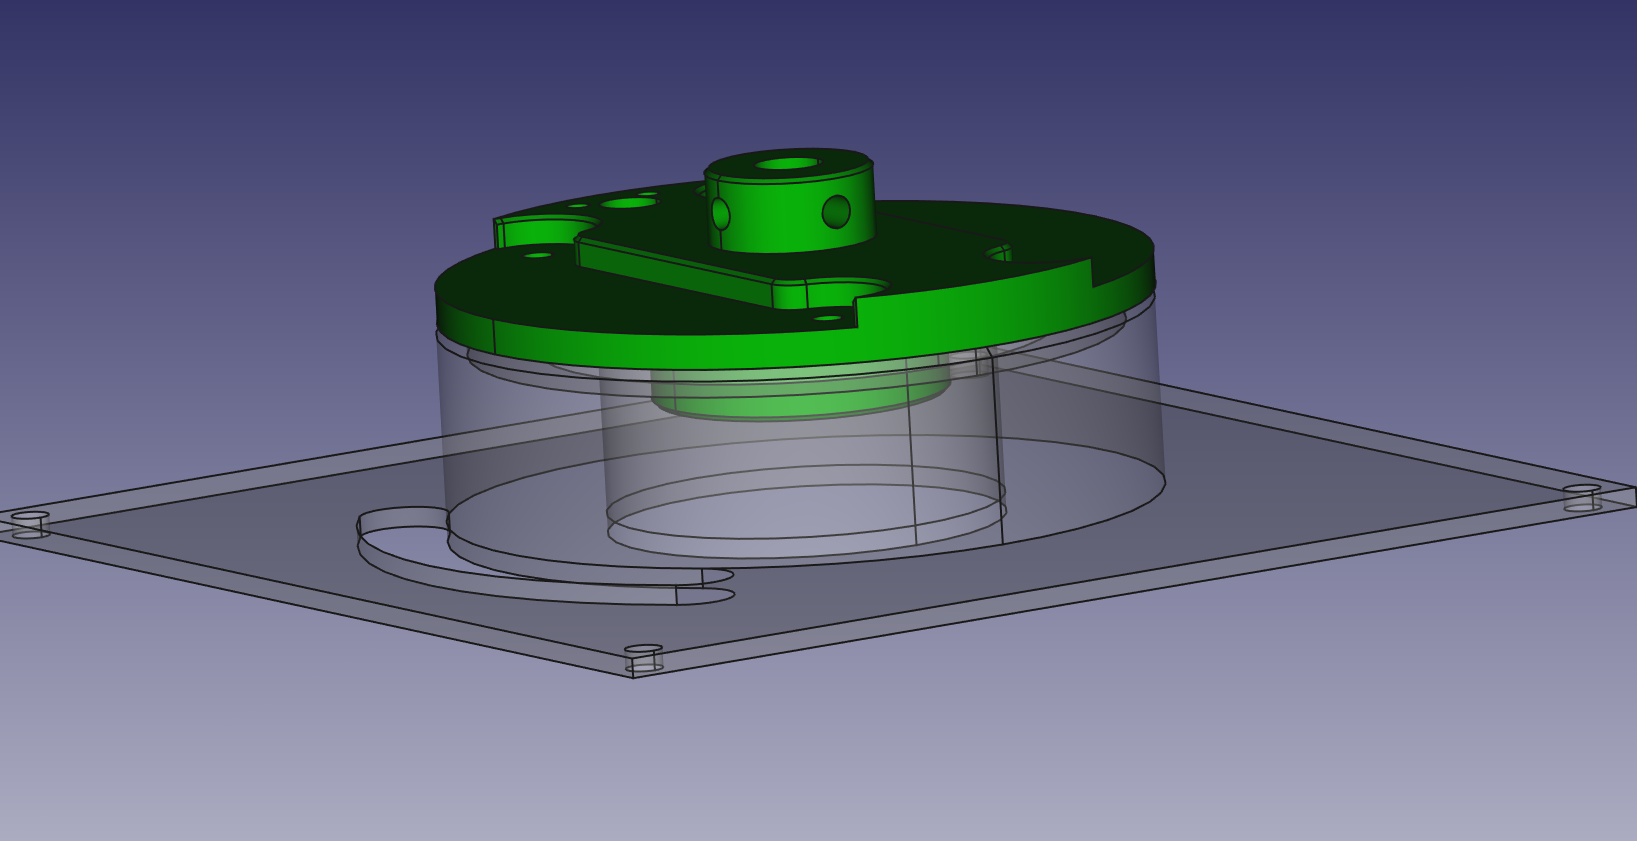
\includegraphics[width=.9\linewidth]{pictures/TapaSuperiorConDisco.png}
    \caption{Tapa superior transparente y base giratoria (verde)}
    \label{fig:tapas_caja_con_disco}
\end{figure}

De esta manera se consigue que el peso de la parte móvil del brazo descanse sobre la tapa y no sobre el eje de rotación. Por otro lado, el hecho de que la base giratoria protruya hacia el interior de la tapa permite que la pieza este mas cerca del motor permitiendo acortar el eje.

A en la figura \ref{fig:cilindro_con_pletina} se muestra la pieza que conecta el motor a la base giratoria a través de un eje. Esta pieza tiene en su base un desgaste tal que permite que el engranaje del motor pueda ser introducido dentro, mientras que en la parte de arriba tiene unos agujeros que permiten la sujeción de un eje metálico el cual llega hasta la base giratoria y transmite el movimiento del motor a esta.

La pieza plana que sale hacia un lateral sirve para que el cilindro pueda alcanzar un fin de carrera que indique cuando el motor ha llegado a una posición extrema.

\begin{figure}[H]
    \centering
    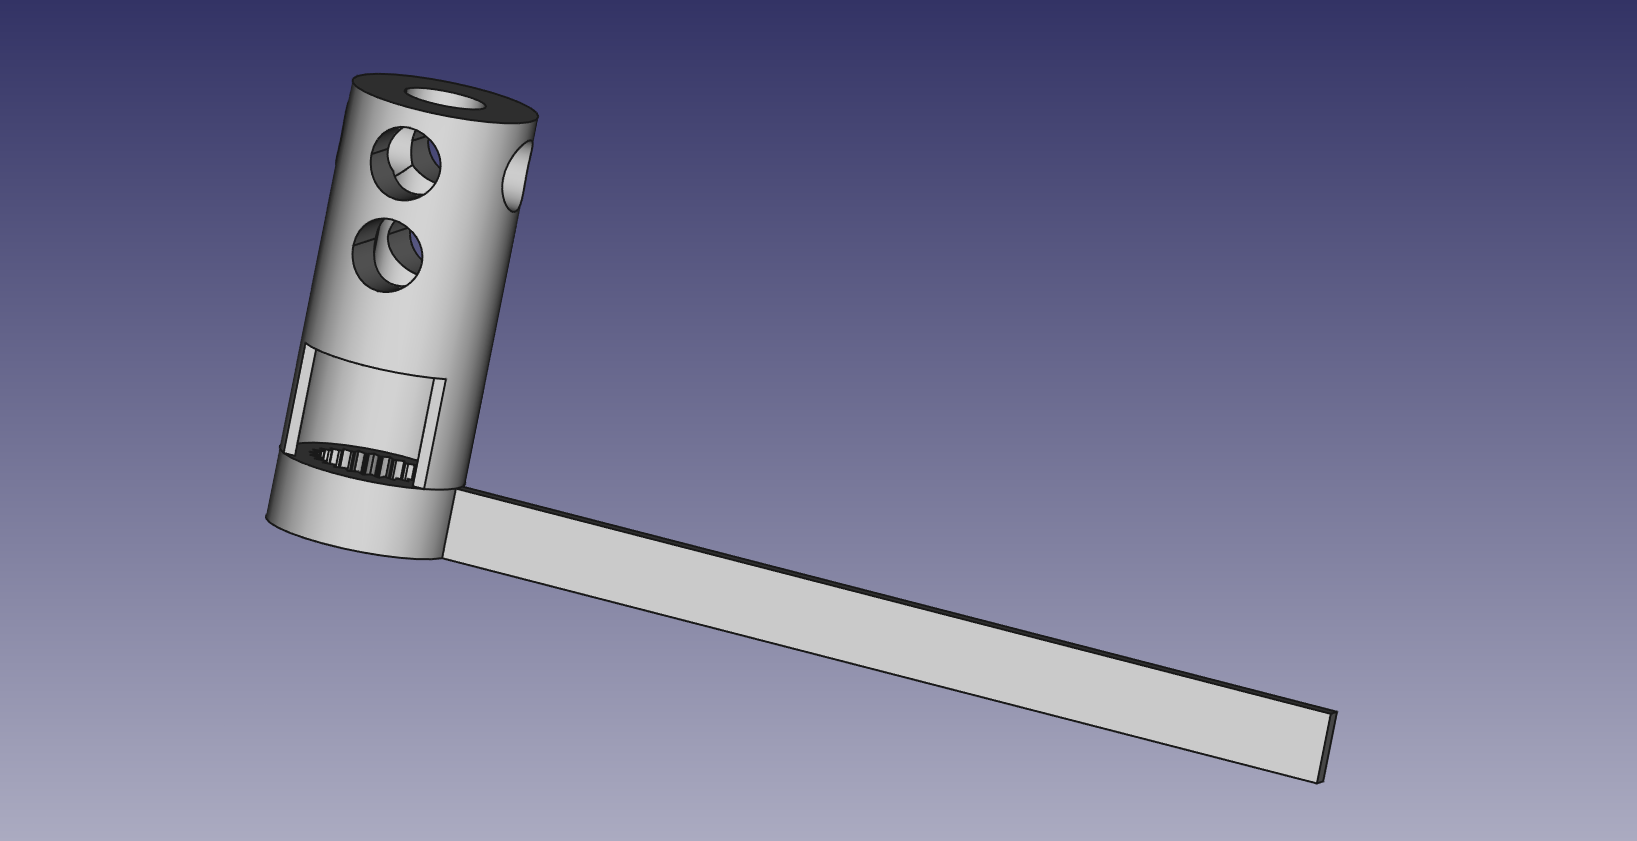
\includegraphics[width=.9\linewidth]{pictures/CilindroConPletina.png}
    \caption{Pieza de unión del motor y el eje}
    \label{fig:cilindro_con_pletina}
\end{figure}

\begin{figure}[H]
    \centering
    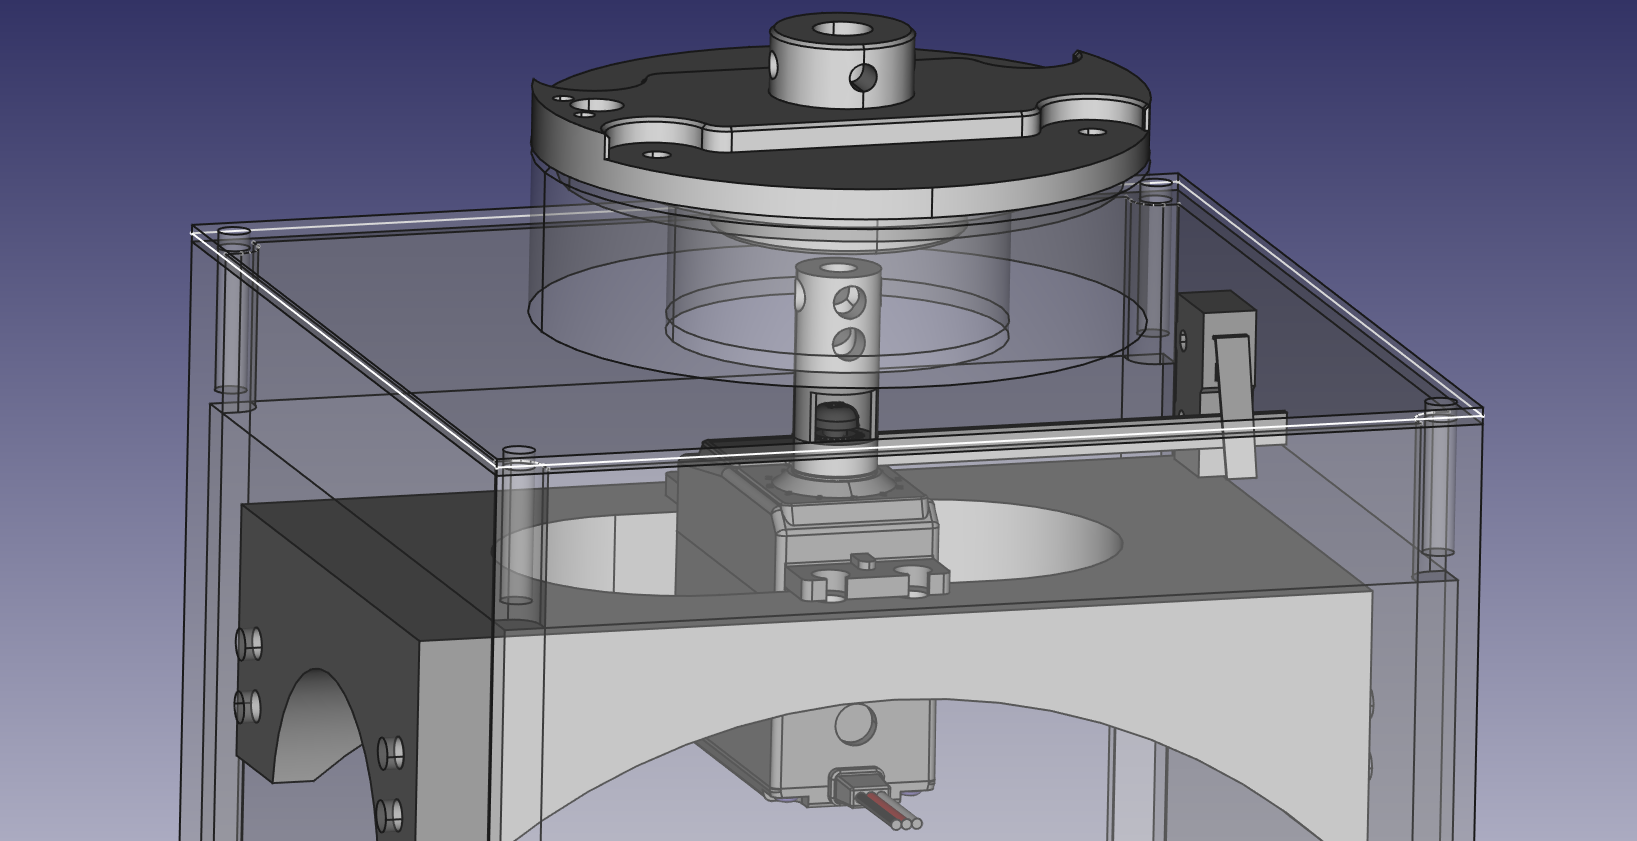
\includegraphics[width=.9\linewidth]{pictures/SistemaCompleto.png}
    \caption{Sistema completo}
    \label{fig:sistema_completo}
\end{figure}

En la figura \ref{fig:sistema_completo} se observa la construcción completa de la base. En esta imagen se dejan las paredes y la tapa superior con cierta transparencia para poder ver el interior de la caja. Entre el cilindro montado encima del motor y la base giratoria habrá un eje metálico que comunicara el movimiento.

Por otro lado, para que sea posible ubicar los motores que se encargaran del movimiento vertical del brazo se han de crear nuevas piezas en las que puedan ser atornillados. Esta pieza puede observarse en la figura \ref{fig:pletina_sujecion_motor}

\begin{figure}[H]
    \centering
    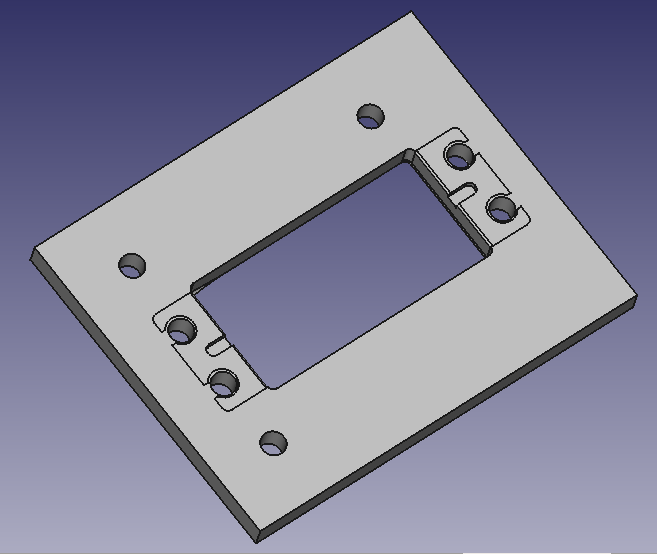
\includegraphics[width=.9\linewidth]{pictures/pletina_motor.png}
    \caption{Placa de sujeción de los motores laterales}
    \label{fig:pletina_sujecion_motor}
\end{figure}

Tras añadir dichas piezas al diseño general y completar este con las piezas originales que no han sido modificados obtenemos el diseño definitivo del brazo robotico el cual se puede observar en la figura \ref{fig:brazo_completo_modificado}.

\begin{figure}[H]
    \centering
    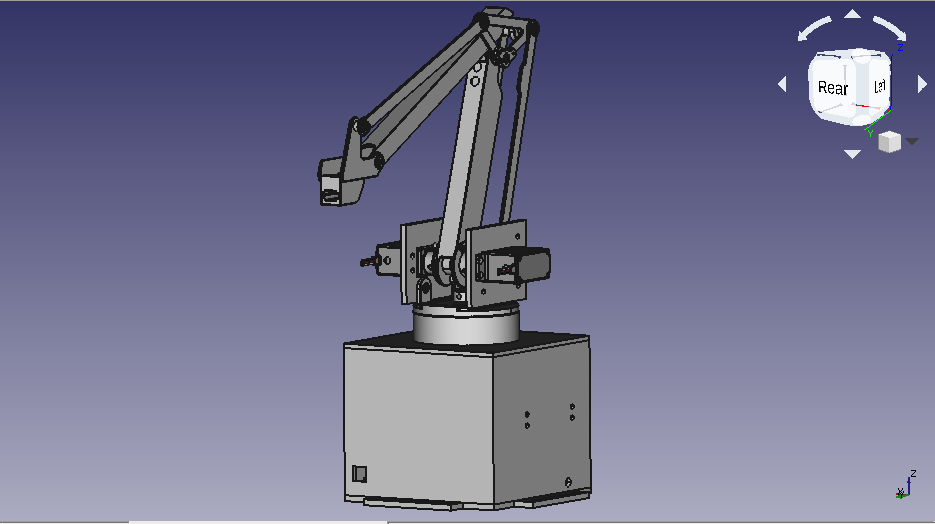
\includegraphics[width=.9\linewidth]{pictures/BrazoEntero.png}
    \caption{Brazo robotico completo tras las modificaciones}
    \label{fig:brazo_completo_modificado}
\end{figure}